% Remove the oneside option below for double sided printing (e.g. for final (post-viva) submission)
\documentclass[a4paper,12pt,oneside,openright]{book}

% Preamble commands go here
\usepackage{customisations}
\usepackage[Bjornstrup]{fncychap}


%% Some of the below packages may be useful to thesis writers in Physics
%% Googling `latex <packagename>' will usually give you some documentation
% \usepackage[load-configurations=abbreviations]{siunitx} % siunitx typesets physical units in a consistent manner
\usepackage{booktabs} % booktabs provides professional formatting commands for tables
\usepackage{amsmath} % amsmath provides extra maths symbols
\usepackage{textcomp} % textcomp provides extra text symbols (like a degrees celsius symbol)
\usepackage{xcolor}
\usepackage{slashed}

\usepackage{graphicx}
\usepackage{float}
\usepackage{afterpage}
\usepackage{amssymb}
\usepackage{multirow}
\usepackage{url}
\usepackage{float}
\usepackage{afterpage}
\usepackage{url}
\usepackage{tikz}
\usetikzlibrary{arrows}
\usepackage{tikz-3dplot}
\usepackage{enumitem}
\usepackage{tabularx}
\usepackage[compat=1.1.0]{tikz-feynhand}
\usepackage{tikz-feynman}
\tikzfeynmanset{compat=1.0.0}



% \usepackage{tikz} % tikz is a package for drawing diagrams and adding annotations to figures
% \usepackage{threeparttable} % threeparttable allows for adding notes to tables
% \usepackage{eps2pdf} % eps2pdf allows background transformation of eps files to pdfs so they 
%						work seamlessly with pdflatex. If using this with the LaTeX editor Kile,
%						you need to add --shell-escape before '%source', in
%						Settings -> Configure Kile... -> Tools -> Build -> build_pdflatex


\graphicspath{{./chapter2/figs/}{./chapter3/figs/}}

\newcommand{\comment}[1]{\textbf{\textcolor{red!90!black}{[#1]}}}
\newcommand{\lp}{\left(}
\newcommand{\rp}{\right)}
\newcommand{\bare}{{(0)}}
\newcommand{\sym}{\mathrm{sym}}
\newcommand{\asy}{\mathrm{asy}}
\newcommand{\as}{\alpha_s}
\newcommand{\nsv}{\mathrm{V}_3}
\newcommand{\nst}{\mathrm{T}_3}
\newcommand{\eg}{{\em e.g.}}
\newcommand{\ie}{{\em i.e.}}
\def \z{\zeta}
% End preamble

% REPLACE THESE with your thesis title, your name and the date of submission of the thesis
\title{Towards a new generation of Parton Distribution Functions: from high-precision collider data to lattice QCD}
\author{Tommaso Giani}
\date{February 2021} % of submission

\begin{document}

% Thesis front matter - title page, abstract, acknowledgements, declaration and table of contents
% See customisations.sty to modify the title page or declaration
\singlespacing
\maketitlepage
\frontmatter
\eighteenptleading
\chapter*{Abstract}
A precise understanding of the proton structure, encoded in Parton Distribution Functions (PDFs), is required 
to make reliable predictions and analyses at the Large Hadron Collider (LHC), 
the main source of experimental data probing subnuclear interactions we have today.
PDFs have played a central role in the recent 
discovery of the Higgs boson and, since it is increasingly clear that any effect due to new physics 
will manifest itself as small deviations from the current theory, 
a precise determination of PDFs is likely to be a key ingredient 
for new physics studies.
%
The PDFs are formally defined as matrix elements of renormalized operators in Quantum Chromodynamics (QCD) involving hadronic states.
They are inherently non-perturbative quantities, and they are extracted from global QCD analysis over
experimental data using the so-called factorization theorems. 
Producing a new generation of PDFs, satisfying the precision and reliability requirements demanded by the current research,
is a challenging task which involves, together with the experimental data input, the development of robust
fitting methodologies, along with new physical ideas. 
%
In this thesis I present a number of progresses which have been developed in the last few years in the context of 
PDFs determination, some of which will lead to the next PDFs release by the NNPDF collaboration. 
In particular I will discuss a new framework for global PDFs determinations, the impact of new experimental data,
with particular emphasis on jets data, the inclusion of theory uncertainty in a PDFs fit 
and the treatment of heavy quarks distributions.
%
I will then discuss a set of recent ideas which would allow to extract PDFs from equal time correlators computable 
within the framework of lattice QCD, and I will present results regarding data coming from different 
lattice approaches and collaborations.

\blankpage


\clearpage
\newpage
\tableofcontents
\mainmatter
\addcontentsline{toc}{chapter}{Introduction}
\chapter*{Introduction}
The increasing demand for accuracy required nowadays to perform high-energy phenomenology
represents one of the main challenge for the particle theory community. The
overall precision of theoretical computations has to match the one of the corresponding
experimental measurements: more precise  
experimental data call for more precise computations, together with a better control
and understanding of the different sources of errors affecting theoretical predictions. 

The computations of high-energy processes involving nucleons are based on factorization, namely on the separation
of amplitudes or cross-sections in different contributions, each of which depends on a specific energy scale.
While short-distance (or high-energy) contributions can be computed within the framework of perturbation theory,
those related to long-distance phenomena and responsible for the internal
structure of the nucleons are not directly accessible by mean of first principle computations, 
and are factorized into universal objects of non perturbative origin, denoted as Parton Distribution Functions (PDFs).
 
PDFs encode our knowledge about the structure of the nucleons in terms of quarks and
gluons, and represent an essential ingredients to perform theory computations in collider physics.
Using factorization theorems, PDFs can be extracted from global QCD fits
over a set of experimental data, and, thanks to their universality, the results can be subsequently used
to compute different processes. 
Unfortunately, they also represent the dominant source of uncertainty in many important computations,
including analyses at the Large Hadron Collider (LHC) and other experiments,
the determination of standard model parameters, Higgs boson characterisation and searches for New Physics.
It is therefore necessary to push the determination of PDFs to a new level of accuracy,
researching for new methodologies and physical ideas to improve such global analyses.

The problem of PDFs determination involves a number of different lines of research which can be investigated 
using diverse approaches.
%
For phenomenological applications, it is important to develop frameworks which allow to implement and test
different numerical and analytical techniques to deal with complex global fits involving a big number of data coming
from experimental measurements. Such frameworks need to be flexible enough in order to fit the available data 
while imposing known physical constraints which have to be satisfied by the final PDFs,
and should allow to easily include new data and computations in the analysis. 
%
When new experimental data for specific high-energy processes become available,
their impact on parton distributions needs to be studied and quantified, to see how the new experimental 
information changes our knowledge regarding the structure of the nucleons.
This involves, on one side, the understanding of the details of the new data (distributions to be included in the analysis,
statistical and systematic errors, kinematic cuts to apply in order to use factorization theorems in their domains of validity), 
on the other the implementation of the most up to date theoretical computation for the process considered.  
%
In order to quantify how reliable the theory predictions are, specific studies regarding the theoretical errors
and their propagations into PDFs need to be carried out, and a suitable prescription for the combination
of experimental and theoretical uncertainties have to be formulated.
%
Alongside this kind of studies, which are usually performed within the high-energy community,
other approaches to study parton distributions are possible.
Being non-perturbative objects, PDFs are also a natural subject for a lattice QCD investigation. 
Starting from the formal definition of parton distributions, given in terms of matrix elements between 
nucleons states of QCD bilocal operators, it is possible to study the detailed structure of the ultraviolet (UV)
and infrared (IR) divergences of such objects, and relate them to specific correlators which, in principle, 
can be obtained through lattice QCD simulations. Such ideas have been studied and developed in recent years,
and data from lattice QCD simulation have started appearing. 
Given the high interest shown by both the lattice and high-energy community, new data for different lattice observables
are likely to appear in the coming years. 
It is therefore important to understand how to extract information about PDFs from them, 
study their potential for high-energy phenomenology,
their interplay with experimental data and understand the different sources of uncertainties 
affecting the corresponding lattice simulation.

This thesis can be divided into three main parts. The first part, composed by the first two chapters, 
is devoted to review the basics of QCD and the main concepts underlying factorization theorems. 
We will introduce parton distributions first from a phenomenological point of view, following the parton model ideas and
discussing the general structure of the NLO QCD corrections, and subsequently following a more formal approach,
revising the theoretical definition of PDFs in terms of QCD bilocal operators.
These chapters are based on a number of standard QCD text books~\cite{Ellis:1991qj,Muta:2010xua,Collins:1984xc},
quantum field theories lectures and classical references regarding factorization in high-energy processes,
such as Refs.~\cite{Collins:1980ui, Collins:1981uw, Collins:1989gx}, and will be used to set up the 
main notations adopted in the rest of the thesis.
%
In the second part, made by chapters~\ref{ch:nnpdf_methodology},~\ref{ch:jets},~\ref{ch:th_error} and ~\ref{ch:bottom}, 
we will present a number of phenomenological studies, as detailed in the following.
%
In chapter~\ref{ch:nnpdf_methodology} we will describe the fitting methodology which has been developed
within the NNPDF collaboration and its recent implementation within the new {\tt n3fit} framework, 
with particular emphasis on the numerical techniques adopted to impose physical constraints on PDFs.
We will also discuss the so called fit basis, showing how
the final results produced within this framework only depend on the experimental and physical inputs, 
and not on the specific details of our fitting methodology. Such studies will be part of the next public release
of the NNPDF collaboration.
%
In chapter~\ref{ch:jets} we will discuss the impact of jets data in a global PDFs determination. 
This gives an example of the kind of analyses which need to be done
every time an important class of new experimental measurements is available, together with the corresponding
theoretical predictions. 
The results discussed in this chapter have been first presented in Ref.~\cite{AbdulKhalek:2020jut}.
In chapter~\ref{ch:th_error} we will discuss the definition and implementation of a theoretical error 
accounting for missing higher orders in a PDFs global analysis. 
The chapter is based on Refs.~\cite{AbdulKhalek:2019bux,AbdulKhalek:2019ihb} where this
study was first presented by the NNPDF collaboration.
In chapter~\ref{ch:bottom}, based on Ref.~\cite{Forte:2019hjc}, we discuss an alternative treatment for the bottom PDFs,
analysing the specific case of Higgs production in bottom fusion and its potential impact on precise phenomenology. 
%
Finally, in the third part of the thesis, made by chapters~\ref{ch:scalar_model},~\ref{ch:qpdfNNPDF} and~\ref{ch:ppdf_NNPDF}, 
we will present a number of studies to understand the relation between PDFs and lattice computable
Euclidean correlators.
In particular in chapter~\ref{ch:scalar_model}, based on Ref.~\cite{DelDebbio:2020cbz},
we will revise the main theoretical ideas behind the lattice approach
using a nongauge theory as a simple toy example. This chapter is used to introduce the theoretical framework necessary
to understand the studies presented in the two following chapters.
In chapter~\ref{ch:qpdfNNPDF} we analyse data for quasi-PDFs matrix elements, studying their potentiality
in constraining PDFs and presenting a detailed analysis of the systematic uncertainties affecting the data and of how
these affect the final results. The results reported in this chapter were first presented in Ref.~\cite{Cichy:2019ebf}.
In chapter~\ref{ch:ppdf_NNPDF} we present results for PDFs extracted from a different kind of lattice 
observables, denoted as reduced Ioffe-time pseudodistribution, assessing differences and similarities with
the analysis of chapter~\ref{ch:qpdfNNPDF}. The chapter is based on Ref.~\cite{DelDebbio:2020rgv}.
Finally in chapter~\ref{ch:conclusions} we briefly summarize the main results and conclusions of this thesis. 

The thesis is supplemented with a number of Appendices, where some analyses are further expanded and 
the details and results of the more technical computations are reported for references. 





\chapter{Basics of QCD}
In the early '60s it was generally believed that a theory for the strong interaction could not be formulated
within the framework of Quantum Field Theory (QFT) \cite{tHooft:1998qmr}.
Despite the remarkable success of Quantum Electrodynamics (QED) in describing phenomena such as the anomalous magnetic moment of the electron,
the renormalization process was not completely understood yet and 
renormalizable quantum field theories were still looked at with suspicion.
 
%
The experimental observation of Bjorken scaling \cite{PhysRev.179.1547} in Deep Inelastic Scattering (DIS) experiment (SLAC 1960)
suggested that the constituents of nucleons may be described as almost-free and point-like objects 
when observed with high spatial resolution, leading to the formulation of the parton model \cite{PhysRevLett.23.1415}.
Accordingly, the dynamic of  partonic systems should have the property of becoming weaker at shorter distances. 
In 1973 asymptotic freedom of non-Abelian gauge field theories was discovered \cite{PhysRevLett.30.1346, PhysRevLett.30.1343},
making possible to embed the partonic model ideas within the framework of a renormalizable QFT.
%
Soon after it was shown how non-Abelian gauge field theories are actually the only ones exhibiting such property
in four dimensional space-time \cite{PhysRevLett.31.851} and Quantum Chromodynamics (QCD) emerged as a mathematically 
consistent theory for the strong interaction.  

%
After its formulation, QCD has been successfully used to describe strong interaction processes observed at colliders, and
nowadays it represents one of the cornerstone of the Standard Model. In this chapter we present
a brief overview of QCD, recalling some basic features of the theory and introducing our notation. 
For a more detailed treatment of the basics of QCD we refer to standard QFT and QCD textbook, such
as Refs.~\cite{Ellis:1991qj,Muta:2010xua,Collins:1984xc}.


%%%%%%%%%%%%%%%%%%%%%%%%%%%%%%%%%%%%%%%%%%%%%%%%%%%%%%%%%%%%%%%%%%%%%%%%%%%%%%%%%%%%%%%%%%%%%%%
\section{Lagrangian and its symmetries}
%
Quantum Chromodynamics is a non-Abelian gauge theory based on the gauge group SU(3)$_\text{color}$.
The classical Lagrangian of QCD, describing the interaction of $N_f$ massive spin-$\frac{1}{2}$ quarks
and massless spin-$1$ gluons, is given by
\begin{align}
    \label{eq:QCD_lagrangian}
    \mathcal{L}_{classical} = -\frac{1}{4}F^{A}_{\mu\nu}F^{A\mu\nu} + 
    \sum_{k=1}^{N_f}\,{\overline{\psi}}^{\,k}_a\left(i\gamma^{\mu}D_{\mu} + m_k\right)_{ab}\psi^k_b\,,
\end{align}
with the field strength tensor and the covariant derivative defined as
\begin{align}
    \label{eq:field_strength_thensor}
    &F^{A}_{\mu\nu} = \partial_{\mu} \mathcal{A}^A_{\nu} - \partial_{\nu} \mathcal{A}^A_{\mu} 
    + g \, f^{ABC} \mathcal{A}^B_{\mu}\mathcal{A}^C_{\nu}\,, \\
    \label{eq:covariant_derivateive}
    &D_{\mu} = \partial_{\mu} - i\,g\,T^A \mathcal{A}^{A}_{\mu}\,.
\end{align}
The summation over $k$ runs over all the quark flavours, with
each quark field $\psi^k_a$ belonging to the fundamental representation of the gauge group SU(3)$_\text{color}$ ($a=1,2,3$),
while the gauge field $\mathcal{A}^A_{\mu}$, called gluon, belongs to the adjoint representation
($A=1,2,...,8$). The quantities $g$ and $f^{ABC}$ are the gauge coupling and the SU(3)$_\text{color}$ structure constants
respectively, and $T^A$ are the eight gauge group generators, satisfying
\begin{align}
    \label{eq:algebra}
    &\left[T^A,T^B\right] = i f^{ABC} T^C\,, \\
    \label{eq:normalization_SU3_generators}
    &\text{Tr}\left[T^A T^B\right] = T_R\, \delta^{AB}\,,
\end{align}
with the normalization of the generators conventionally chosen to be $T_R = 1/2$. 
An explicit expression for the generators $T^A$ in the fundamental representation is given by
$(T^A)_{ab} = 1/2\,\left(\lambda^A\right)_{ab}$ with $\lambda^A$ representing the eight 3-dimensional Gell-Mann matrices. 
Given the equations above, the colour matrices obey
\begin{align}
    \label{eq:SU3_generators_relations}
    &\sum_A T^A_{ab} T^A_{bc} = C_F\, \delta_{ac}\,,\\
    &\sum_{C,D} T^A_{CD} T^B_{DC} = \sum_{C,D} f^{ACD} f^{BCD}  C_A\, \delta^{CD}\,,
\end{align}
with $C_F= 4/3$ and $C_A= 3$.

%
The classical Lagrangian of Eq.~\eqref{eq:QCD_lagrangian} does not allow to formulate quantum
perturbation theory in a consistent way. The problem cannot be avoided as long as
we rely on a gauge invariant Lagrangian, where the gauge field $\mathcal{A}^A_{\mu}$
has the freedom to change according to gauge transformations.
We can get rid of such freedom by putting constraints on the field $\mathcal{A}^A_{\mu}$, 
known as \textit{gauge fixing conditions}, which in general can be expressed as
\begin{align}
    \label{eq:gauge_fixing}
    G^{\mu}\mathcal{A}_{\mu}^A = B^A\,,
\end{align}
with $G^{\mu}$ and $B^A$ chosen in some convenient way. 
Upon functional integration over the arbitrary quantity $B^A$, such condition is implemented 
in the theory by adding to the classical Lagrangian the so-called gauge fixing term
\begin{align}
    \label{eq:Gauge_fixing_lorents}
    \mathcal{L}_{gauge-fixing} = -\frac{1}{2\xi}\left(G^{\mu}\mathcal{A}_{\mu}^A\right)\,,
\end{align}
with $\xi$ representing an arbitrary parameters whose specific values defines the gauge.
Different choices for the gauge fixing term can be done. Taking $G^{\mu}=\partial^{\mu}$ we obtain
a class of covariant gauges. In this case the gauge fixing term must be supplemented by an additional term,
known as \textit{ghost Lagrangian} \cite{Faddeev:1967fc},
describing a complex scalar field $\eta^a$ (the Faddeev-Popov ghosts) obeying the Grassmann algebra and belonging to the adjoint
representation of the gauge group
\begin{align}
    \label{eq:ghosts_lagrangian}
    \mathcal{L}_{ghost} = \left(\partial_{\alpha}\eta^A\right)^* D^{\alpha}_{AB}\, \eta^B\, .
\end{align}
Perturbation theory can be formulated starting from the Lagrangian density
\begin{align}
    \label{eq:QCD_lagrangian_gauge_fixing}
    \mathcal{L} = \mathcal{L}_{classical} + \mathcal{L}_{gauge-fixing} + \mathcal{L}_{ghost}\, .
\end{align}
Another possible gauge fixing term is the one giving the so called axial gauges, fixed
in terms of a chosen vector $n$ such that $G^{\mu}=n^{\mu}$. In this case ghost fields decouples
and can thus be ignored, but the explicit form of the gluon propagator turns out to be more complicated than 
the one in the covariant gauges.

The QCD Lagrangian has a number of important symmetries, both exact and approximate,
which is worth recalling here.
The classical Lagrangian given in Eq.~\eqref{eq:QCD_lagrangian} is invariant under SU(3)$_{\text{color}}$
gauge transformations. After gauge fixing gauge invariance is broken, but the resulting Lagrangian of 
Eq.~\eqref{eq:QCD_lagrangian_gauge_fixing} satisfied the BRST symmetry \cite{Becchi:1975nq, Tyutin:1975qk},
which in turn guarantees the renormalizability of the theory.
The so called flavour symmetries are also exact symmetries of QCD, 
acting through a global phase transformation of each quark field separately and giving
the baryon number conservation. 
%the conservation of the number of each of the different quark flavours. 
Other flavour symmetries include the discrete global symmetries of parity and time reversal invariance.
Finally charge-conjugation is also an exact symmetry of Eq.~\eqref{eq:QCD_lagrangian_gauge_fixing}. 

Assuming mass degeneracy for the up and down quarks, the U(1) global symmetry associated with quark number 
can be extended to a global U(2) $=$ U(1) $\otimes$ SU(2). The new symmetry SU(2) is known as isospin symmetry.
We can further enhanced the symmetry group to U(1) $\otimes$ SU(3) assuming the strange quark to be also 
degenerate in mass with the up and the down\footnote{Such approximate flavour symmetry SU(3) is the basis of the Gell-Mann
quark model \cite{GellMann:1964nj} which was proposed well before the birth of QCD.}.
In the case of massless quarks, a chiral symmetry
U(2)$_{L}$ $\otimes$ U(2)$_R$ $=$ SU(2)$_V$ $\otimes$ U(1)$_V$ $\otimes$  SU(2)$_A$ $\otimes$ U(1)$_A$ 
holds, which however is spontaneously broken to SU(2)$_V$ $\otimes$ U(1)$_V$ $\otimes$ U(1)$_A$,
with the subscripts $V$ and $A$ denoting the vector and axial combinations.
The three pseudo-scalar Goldstone bosons resulting from chiral SU(2) breaking 
to SU(2)$_V$ are identified with the three pions $\pi^+$, $\pi^-$ and $\pi^0$
in the massless quark limit. 
While the survived SU(2)$_V$ $\otimes$ U(1)$_V$ symmetry is identified with the isospin and baryon number 
conservation mentioned previously, the remaining U(1)$_A$, despite not being spontaneously broken,
appears to be lost in QCD. The study of what happens to this symmetry is known as the U(1)-problem~\cite{Weinberg:1975ui}.
The axial symmetry U(1)$_A$ is actually broken at the quantum level, through the Adler-Bell-Jackiw anomaly,
which induces a new term in the QCD Lagrangian proportional to 
$\epsilon_{\alpha\beta\gamma\delta}\, \text{Tr}\, F^{\gamma\delta} F^{\alpha\beta}$ .
This term would be responsible for a violation of CP in the strong sector and 
its magnitude is given by the size of the parameter $\theta$, whose values is fixed to be in the range
$\theta<10^{-9}$ by experimental measures. The unexplained smallness of such parameter is known as the strong CP-problem.
Among the proposed solutions, the Peccei-Quinn mechanism was developed \cite{Peccei:1977ur}, proposing a dynamical explanation
for the $\theta$ values through the introduction of additional particles called axions. 

%%%%%%%%%%%%%%%%%%%%%%%%%%%%%%%%%%%%%%%%%%%%%%%%%%%%%%%%%%%%%%%%%%%%%%%%%%%%%%%%%%%%%%%%%%%%%%%
\section{The running coupling and asymptotic freedom}
%
In analogy with the QED fine structure constant,
the QCD coupling constant is defined in terms of the gauge coupling as $\alpha_s = g^2/4\pi$.
As a consequence of the renormalization process, the coupling acquires a dependence on the renormalization scale $\mu$,
namely the arbitrary scale at which the subtraction of the ultraviolet (UV) poles is performed. 
The resulting renormalization group equations read
\begin{align}
    \label{eq:renormalization_group_coupling}
    \mu^2\frac{\partial\alpha_s}{\partial \mu^2} = \beta\left(\alpha_s\right)\,.
\end{align}
The $\beta$ function can be computed in perturbation theory as a power expansion in $\alpha_s$. 
Nowadays results up to five loops have been computed \cite{Herzog:2017ohr}.
At next-to-leading order it is given by
\begin{align}
    \label{eq:beta_function_expansion}
    \beta\left(\alpha_s\right) = -\beta_0\,\alpha_s^2\left(1+ \beta_1 \alpha_s + \mathcal{O}\left(\alpha_s^2\right)\right)\,,
\end{align}
with
\begin{align}
    \label{eq:beta_function_coefficients}
    \beta_0 = \frac{33 - 2 N_f}{12\pi}\,,\,\,\,\,\,
    \beta_1 = \frac{153 -19 N_f}{2\pi\left(33-2 N_f\right)}\,.
\end{align}
Using the leading order expression for the $\beta$ in Eq.~\eqref{eq:renormalization_group_coupling} we find the leading-log
solution for the running coupling, relating its value at the generic scale $Q^2$ to the one at a reference scale
$\mu^2$ 
\begin{align}
    \label{eq:ll_coupling}
    \alpha_s\left(Q^2\right) = \frac{\alpha_s\left(\mu^2\right)}{1+\alpha_s\left(\mu^2\right)\beta_0\log\frac{Q^2}{\mu^2}}\,.
\end{align}
Given the positive sign of $\beta_0$, from Eq.~\eqref{eq:ll_coupling} it is evident how, as the scale $Q^2$ becomes very large, 
the coupling $\alpha_s\left(Q^2\right)$ decreases to zero. This property, which characterizes non-Abelian gauge theories 
like QCD, is known as asymptotic freedom and the theory is then said to be asymptotically free.
It is customary to introduce a dimensionful parameter, usually denoted as $\Lambda_{\text{QCD}}$, representing the energy 
scale at which the perturbative series of the coupling would diverge
\begin{align}
    \label{eq:lambda_QCD}
    \frac{1}{\alpha_s\left(\Lambda_{\text{QCD}^2}\right)} = 0\,.
\end{align}
Its specific value will depend on the choice of the renormalization scheme, on the order
of the $\beta$ function power expansion and on the number of active flavours\footnote{the notion of active flavours will
be discussed in Sec.~\ref{sec:quark_masses}} entering the theory.
Qualitatively it represents the scale at which the interaction becomes strong and the perturbative description breaks down.

\section{Quark masses}
\label{sec:quark_masses}
The quark masses represent another parameter of the Lagrangian Eq.~\eqref{eq:QCD_lagrangian}.
Just like the coupling constant because of the renormalization process they also acquire a
dependence on a renormalization scale $\mu$ given by 
\begin{align}
    \label{eq:renormalization_mass}
    \mu^2\frac{\partial m }{\partial \mu^2} = - \gamma_m\left(\alpha_s\right)m\left(\mu^2\right)\,.
\end{align}
The quantity $\gamma_m$ is the mass anomalous dimension which can computed in perturbation theory as
a power expansion in $\alpha_s$
\begin{align}
    \gamma_m\left(\alpha_s\right) = c\,\alpha_s\left(1+c'\alpha_s + ...\right)\,,
\end{align}
with the explicit expression of the coefficients depending on the choice of the renormalization scheme.

%
In order to study the impact of the quarks mass on a generic physical observable $R$, let's consider
the situation in which we have only one quark with mass $m$.
Writing $R = R\left(Q^2/\mu^2, \alpha_s\left(\mu^2\right),m\left(\mu^2\right)/Q \right)$ 
and setting the renormalization scale equal to the physical scale $\mu=Q$,
if we assume the first $N$ derivatives of $R$ to be finite in $m=0$ 
we can write the expansion
\begin{align}
    \label{eq:R_mass_dependence}
    R&\left(1, \alpha_s\left(Q^2\right),m\left(Q^2\right)/Q \right) \sim
    R\left(1, \alpha_s\left(Q^2\right),0 \right)\nonumber \\
    & + \sum_{n=1}^{N}\frac{1}{n!}\left[\frac{m\left(Q^2\right)}{Q^2}\right]^n R^{(n)}\left(1,\alpha_s\left(Q^2\right),0\right)\,.
\end{align}
where $R^{(n)}$ denotes the $n$-th derivative of $R$ with respect to its third argument. 
Given the fact that Eq.~\eqref{eq:renormalization_mass} leads to a change of the renormalized mass with $Q$ 
which is at most logarithmic, from Eq.~\eqref{eq:R_mass_dependence} it is clear how, when considering 
high energy scales $Q \gg m$, the mass dependence can be dropped, and the quark can be considered massless.
%
On the other hand, when the mass of the quark is much greater of the relevant scale $Q$ it can be shown 
that the heavy quark mass correction to $R$ are suppressed by inverse powers of $m$, and therefore they can be ignored when
$Q \ll m$. 
%
The $n_l$ active flavour introduced in the previous section are the light quarks whose mass is much smaller than
the physical scale $Q$.

%
Considering the situation in which we have $n_l$ light quarks (i.e. quarks whose mass is much smaller than $Q$)
and a single heavy quark with mass $m$, the two values $\alpha_s^{(n_l+1)}$ and $\alpha_s^{(n_l)}$ 
measured in the two domains $Q \gg m$ and $Q \ll m$ respectively,
are usually matched requiring  the coupling $\alpha_s\left(Q^2\right)$
to be continuos at $Q=m$, getting a matching equation of the form
\begin{align}
    \alpha_s^{(n_l+1)}\left(Q^2\right) = 
    \alpha_s^{(n_l)}\left(Q^2\right) 
    + \sum_{k=2}^{\infty} c_k\left(L\right) \left(\alpha_s^{(n_l)}\left(m^2\right)\right)^k\,,
\end{align}
where the coefficients $c_k\left(L\right)$ are  polynomials in $L=\log Q^2/m^2$.
Depending on the specific energy scale of interest,
one can perform the computation of a generic physical observable considering either $n_l$ or $n_l + 1$ active flavours,
each choice being more convenient in a given kinematic region. 
In Sec.~\ref{sec:fonll} we will discuss a way in which such computations can be combined in a unique result which
is accurate at every energy scale.

%%%%%%%%%%%%%%%%%%%%%%%%%%%%%%%%%%%%%%%%%%%%%%%%%%%%%%%%%%%%%%%%%%%%%%%%%%%%%%%%%%%%%%%%%%%%%%%
\section{Perturbative and non-Perturbative approaches}
The property of asymptotic freedom allows to compute high energy scattering processes as
an expansion in the coupling, paving the way to a perturbative treatment of QCD.
The Lagrangian given in Eq.~\eqref{eq:QCD_lagrangian_gauge_fixing}
can be written as the sum between the free Lagrangian $\mathcal{L}_0$, describing free fermions and gauge fields, 
plus an interaction term $\mathcal{L}_I$, containing all the terms proportional to the gauge coupling $g$:
at high energy $g$ becomes small, and all these terms 
can be treated as perturbative interactions, so that the corresponding
contribution in the action can be expanded in a power series of the coupling.

%
In general, perturbation theory can be seen as a systematic way of approximating the solution 
of a quantum field theory keeping the error under control.
Although its success in describing high energy processes, it is not a full solution of the theory, 
and there are situations in which it cannot be applied: in the case of QCD, at low energy the coupling
becomes large, and a power expansion in $\alpha_s$ is no longer possible. 
It is therefore important to have a non-perturbative formulation of QCD, based on the classical Lagrangian 
of Eq.~\eqref{eq:QCD_lagrangian}.
The framework of lattice QFT represents one of the most studied and developed systematic approaches to study quantum
field theories in non-perturbative regimes. In the following we recall the basic ideas underlying the formulation of 
QCD on an Euclidean lattice, referring to standard textbooks as Ref.~\cite{smit_2002} for a complete discussion.

%
In lattice QFT the path integral of the theory is defined on a discrete and finite Euclidean space-time,
characterized by a finite volume and lattice spacing $a$, and directly evaluated through Monte-Carlo simulations.
The lattice can be defined as a cartesian product
\begin{align}
    \label{eq:lattice_def}
    \Lambda^4\left(N\right) = a\Big([\![0, N_0-1 ]\!]\times[\![0, N_1-1 ]\!]\times[\![0, N_2-1 ]\!]
    \times[\![0, N_3-1 ]\!] \Big)\,,
\end{align}
where $N$ is a four vector with integer components and $[\![0, n ]\!]$ is the set of all the integers $j$ such that
$0 \le j \le n$. The integer $N_{\mu}$ represents the number of lattice sites in the $\mu$ direction, corresponding
to a space-time extent equal to $a N_{\mu}$. 
From this definition it is clear how for each point $x_{\mu}$ belonging to the lattice there exists a four vector $j_{\mu}$ 
with integer coordinates such that $x_{\mu} = a j_{\mu}$. 
The zero-component $N_0$ is usually identified with the temporal extent
$T = a N_0$, while the three remaining ones, assumed to be equal, represent the spatial extent in the three spatial directions
$L = a N_1 = a N_2 = a N_3$. On such lattice the full Lorentz invariance of the continuum 
Minkowski space-time is reduced to the hypercubic group, 
however when considering gauge theories their lattice version is built in such a way to preserve gauge invariance. 

Considering for simplicity a theory containing a single scalar field $\phi$,
taking a generic correlation function in Minkowski space 
\begin{align}
    C_n^{(M)}\left(x_1,..., x_n\right) = 
    \frac{1}{Z} \int \phi\left(x_1\right)...\phi\left(x_n\right)\exp\left(i S^{(M)}\left[\phi\right]\right)\,,
\end{align}
one can define the associated Euclidean correlation function
by performing a Wick rotation $x_i = \left(x^0_i, \vec{x}_i\right) \rightarrow \bar{x}_i = \left(-i x^0_i, \vec{x}_i\right)$
\begin{align}
    \label{eq:euclidean_correlator}
    C_n^{(E)}\left(x_1,..., x_n\right) &\equiv C_n^{(M)}\left(\bar{x}_1,..., \bar{x}_n\right) = \nonumber \\
    &\frac{1}{Z} \int \phi\left(x_1\right)...\phi\left(x_n\right)\exp\left(- S^{(E)}\left[\phi\right]\right)\,,
\end{align}
where $S^{(E)}$ is the Euclidean action of the theory.
Such Wick rotation effectively transform the Minkowski metric $\eta_{\mu\nu} = \text{diag}\left(1,-1,-1,-1\right)$
into the positive Euclidean metric $\delta_{\mu\nu} = \text{diag}\left(1,1,1,1\right)$.
The functional integral of Eq.~\eqref{eq:euclidean_correlator} can be estimated
by averaging the fields product $\phi\left(x_1\right)...\phi\left(x_n\right)$ on the probability density 
$D\phi \, \text{exp}\left(-S^{(E)}\left[\phi\right]\right)$ .


%
In order to write a discrete version of QCD, we need to construct an action for the gauge field and one for the quark fields.
In the case of the gauge field, the action can be written in terms of gauge links $U_{\mu}$, obtaining the so called Wilson action
\begin{align}
    \label{eq:Wilson_action}
    &S_G\left(U_{\mu}\right) = 
    \frac{\beta}{N}\sum_{x\in \Lambda^4}\sum_{\mu>\nu}\text{Re}\left(1-P_{\mu\nu}\left(x\right)\right)\,, \\
    &P_{\mu\nu}\left(x\right) = U_{\mu}\left(x\right)U_{\nu}\left(x+a\hat{\mu}\right)
    U_{\mu}\left(x+a\hat{\nu}\right)^{\dagger}U_{\nu}\left(x\right)^{\dagger}\,,
\end{align}
where $\beta$ is a constant of the theory. It can be shown that in the continuum limit Eq.~\eqref{eq:Wilson_action}
recovers the Euclidean Yang-Mills action.

%
Considering the fermionic fields, defining the translation operator in the $\hat{\mu}$ direction as 
$\tau_{\mu}f\left(x\right) = f\left(x+a\hat{\mu}\right)$, 
it turns out that a naive discretization of the Dirac action
\begin{align}
    \label{eq:naive_Dirac}
    S_{\text{Dirac}}\left[\psi,\bar{\psi}\right] = 
    a^4\sum_{x\in\Lambda^4}\bar{\psi}\left(x\right)\left(\frac{\gamma^{\mu}}{2a}\left(\tau_{\mu}-\tau_{-\mu}\right) + m\right) \psi\left(x\right)
\end{align}
would lead to a theory with the wrong continuum limit, describing 16 independent fermion states all having the same energy.
This is the so-called \textit{doubling problem}, and it is a consequence of a more general property of 
fermionic actions known as the Nielsen-Ninomiya no-go theorem~\cite{Nielsen:1981hk}.
A possible solution to the doubling problem was proposed by Wilson~\cite{PhysRevD.10.2445}, through the addition of another term to the fermionic action
to remove the unwanted states
\begin{align}
    \label{eq:fermions_wilson_action}
    S_W\left[\psi,\bar{\psi}\right] = S_{\text{Dirac}}\left[\psi,\bar{\psi}\right] 
    - \frac{a^5}{2}\sum_{x\in\Lambda^4}\bar{\psi}\left(x\right)\tilde{\delta}^2 \psi\left(x\right)\,,
\end{align}
where $\tilde{\delta}^2 = a^{-2}\sum_{\mu}\left(1-\tau_{-\mu}\right)\left(\tau_{\mu}-1\right)$.
In the presence of a gauge field, Eq.~\eqref{eq:fermions_wilson_action} becomes 
\begin{align}
    S_W\left[\psi,\bar{\psi}, U_{\mu}\right] = a^4\sum_{x\in\Lambda^4}\bar{\psi}\left(x\right)\left(K\left[U_{\mu}\right] + m\right)\psi\left(x\right)\,,
\end{align}
where $K\left[U_{\mu}\right]$ is a suitable discretization for the covariant derivative which implements
the Wilson prescription. 
The addition of the Wilson term in the action solves the doubling problem, however it explicitly breaks
chiral symmetry, leading to a more complex UV structure of the theory.

%
Once the Euclidean action has been defined, the expectation value of a generic observable 
$O\left[\psi,\bar{\psi},U_{\mu}\right]$ can be evaluated
through the path integral
\begin{align} 
    \label{eq:lattice_path_integral}
    \langle O\rangle = \frac{1}{Z}\,\int D\psi\, D\bar{\psi}\,DU_{\mu}\,
    O\left[\psi,\bar{\psi},U_{\mu}\right]e^{-S[\psi,\bar{\psi},U_{\mu}]}\,.
\end{align}
with 
\begin{align}
    S[\psi,\bar{\psi},U_{\mu}] = S_G\left(U_{\mu}\right) + S_W\left[\psi,\bar{\psi}, U_{\mu}\right]\,.
\end{align}
Since the fermionic action is quadratic,
the functional integrals over $\psi$ and $\bar{\psi}$ can be performed analytically getting
\begin{align}
    \label{eq:integrated_path_integral}
    \langle O\rangle = \frac{1}{Z}\int DU_{\mu}\,\text{det}\left(K+M\right)
    O_{\text{Wick}}\left[U_{\mu}\right]e^{-S_G[U_{\mu}]}\,,
\end{align}
where $O_{\text{Wick}}$ denotes the functional obtained from $O$ performing the Wick contractions 
of the quark fields. Note that this observable depends on the quark propagator $\left(K+M\right)^{-1}$,
appearing for every $\psi\bar{\psi}$ contraction. Inverting the term $K+M$ in order to obtain the fermionic propagator
represents the elementary computation in lattice QCD simulations.
Assuming $\text{det}\left(K+M\right)>0$ \footnote{in a continuum theory it 
can be shown that this is true thanks to chiral symmetry, as long as we consider non-zero masses.
On the lattice the situation can be more complicated: in the case of Wilson fermions for example chiral symmetry is lost,
and the determinant is positive only when the bare masses are bigger than the critical mass.}, the quantity
\begin{align}
    \label{eq:prob_distribution}
    \frac{1}{Z}\,\text{det}\left(K+M\right)e^{-S_G[U_{\mu}]}\,,
\end{align}
can be interpreted as a probability distribution and an estimation
for $\langle O \rangle$ up to a $\mathcal{O}\left(1/\sqrt{N}\right)$ statistical error can be obtained by drawing
N samples $U_{\mu}^{(i)}$ from it and computing
\begin{align}
    \label{eq:average_O_lattice}
    \langle O \rangle = \frac{1}{N}\sum_{i=0}^N \, O\left[U_{\mu}^{(i)}\right]\,.
\end{align} 

\chapter{Factorization theorems in QCD}
In the previous chapter we have seen how, thanks to asymptotic freedom, the structure of QCD simplifies when considering problems
involving short-distance or high energy scales: the coupling becomes small and the theory can be solved perturbatively.
However, cross sections for high energy processes are usually a combination of short- and long-distance effects, and cannot
be fully computed within the framework of perturbation theory. Factorization theorems allows to separate (factorize) a cross section
or amplitude in separate contributions, each factor containing the dependence of the process on a specific distance scale:
while short-distance effects can be computed in perturbation theory, contributions coming from long-distance phenomena have
to be extracted from experimental data. 
In this chapter, starting from the Parton Model ideas we will discuss factorization theorems in QCD,
using the case of Deep Inelastic Scattering as a basic example. We will then introduce the main subject of the
present work, namely Parton Distribution Functions (PDFs).

%%%%%%%%%%%%%%%%%%%%%%%%%%%%%%%%%%%%%%%%%%%%%%%
\section{The Parton Model}
The basic ideas underlying factorization theorems for high energy processes can 
be described appealing to Feynman's parton model \cite{PhysRevLett.23.1415,Feynman:1973xc, Bjorken:1969ja}.
In this picture fundamental particles called \textit{partons} are bounded together to form hadrons.
Since the details of the partonic system are unknown, the scattering between a test particle and the hadron 
as a whole cannot be computed. However we assume that we do know how to describe the scattering with a free parton.
%
As example, let us consider the case of the scattering of a high-energy charged lepton off a
hadron target 
$$e^{-}(k)\,H\,(P)\,\rightarrow e^{-}(k')\,X \,. $$ 
Such process is known as Deep Inelastic lepton-hadron Scattering (DIS).
Looking at this scattering in the centre of mass frame, the hadron will be Lorentz contracted 
in the direction of the collision and the lifetime of the internal partonic states will be lengthened.
As a consequence, the time the electron takes to cross the hadron will be much shorter than the average lifetime of
each partonic states. During the time of the interaction the hadron can then be thought as "frozen" in 
a well defined partonic states, with each parton carrying a definite fraction $\xi$ of the hadron momentum
and not interacting with the other ones. 
If the energy of the collision is high enough, the virtual photon mediating the electron-hadron 
interaction will interact with a single parton having a given momentum fraction. Likewise, interactions
occurring in the final states are assumed to occur on time scales too long to interfere with the hard scattering.
%
Given this picture, it is natural to think about the scattering cross section as classical and incoherent,
namely as a sum of probabilities rather than of amplitudes. The parton model ideas can be summarized in the simple formula
\begin{align}
    \label{eq:parton_model}
    \sigma&\left(e^{-}\left(k\right)H\left(P\right)\rightarrow e^{-}\left(k'\right)+X\right) = \nonumber\\
     &\,\,\,\,\,\,\,\,\sum_i\int_0^1 d\xi\, q_{i/H}\left(\xi\right)
     \hat{\sigma}\left(e^{-}\left(k\right)q_i\left(\xi P\right)\rightarrow e^{-}\left(k'\right)+q_f\right)
\end{align}
where $\hat{\sigma}$ represents the partonic cross section describing the interaction between 
a single free parton and the virtual photon, and the set of functions $q_{i/H}\left(\xi\right)$ the probability densities
of having a parton of kind $i$ inside the hadron $H$, carrying a fraction $\xi \in \left(0,1\right)$ of the total hadron momentum. . 

%
In the following we recall in more details how parton model ideas apply to the case of 
DIS, setting the stage for a more complete 
discussion of factorization which will be addressed in the next section. % discussing the inclusion of NLO QCD corrections.  
DIS experiments are traditionally the main testing ground of perturbative QCD,
having been the first processes where pointlike particles were seen inside the hadron, 
thus motivating the formulation of the parton model. 
They play a central role in any discussion regarding factorization and provide a simple experimental and theoretical framework to
study the strong interaction.
As we are going to recall in the following, measurements of DIS structure functions directly probe the structure of hadrons, 
giving the bulk of experimental measurements at the basis of every phenomenological determination of Parton Distribution Functions.

\begin{figure}[h!]
    \center
    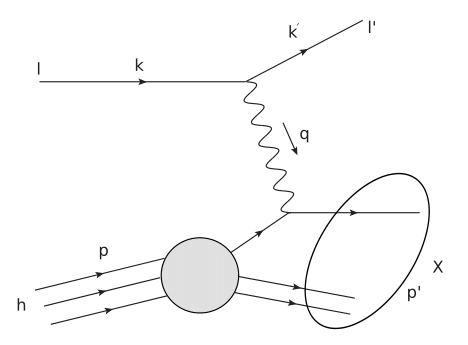
\includegraphics[scale=0.7]{dis.png}
    \caption{DIS kinematic in the parton model.}
    \label{fig:DIS_kin}
\end{figure}

The kinematic for DIS is reported in Fig.~\ref{fig:DIS_kin}.
The space-like momentum of the photon (if the initial lepton is an electron or a muon then the scattering is 
mediated by the exchange of a photon) is given by $q = k - k'$, the centre of mass energy square is $s=\left(P+k\right)^2$ and
we denote the invariant mass square of the finale states as $W = \left(P+q\right)^2$.
It is customary to introduce the kinematic variables
\begin{align}
	\label{eq:DIS_kinematic}
    & Q^2 = -q^2 > 0\,, \,\,\,\,\,\, x = \frac{Q^2}{2P\cdot q}\,, \,\,\,\,\,\, y = \frac{Q^2}{x s}\,.
    %y = \frac{P\cdot q}{P\cdot k }\,.
\end{align}
In the regime 
$$ Q^2,\, W^2 >> m^2_{\text{hadron}} \sim \Lambda^2_{\text{QCD}}\,, $$ 
leptons and quarks masses can be neglected.
It is easy to see that the variable $x$, known as \textit{Bjorken variable} can take values between 0 and 1, 
with $x\rightarrow 1$ representing the elastic limit in which $W=m^2_{\text{hadron}}$. The Deep Inelastic regime
is then defined as $Q^2 >> \Lambda^2_{\text{QCD}} $ with $x$ fixed and different from 1.

%
The corresponding amplitude reads
\begin{align}
    \label{eq:DIS_amplitude}
    \mathcal{M} = 
    \frac{e}{q^2}\bar{u}\left(k'\right)\gamma^{\alpha}u\left(k\right)\langle X | j_{\alpha}\left(0\right)|P\rangle,
\end{align}
where $|X\rangle $ represents the generic final state with $n$ on-shell particles and $j_{\alpha}$ 
is the electromagnetic current through which the photon interacts in the proton.
The cross section, which is proportional to the amplitude square, is then found to be proportional to the product between 
a leptonic and an hadronic part
\begin{align}
    \label{eq:DIS_xsec}
    \frac{d\sigma}{dx\,dQ^2} \propto \int \frac{d^3k'}{2E_{k'}\left(2\pi\right)^3}\, W^{\mu\nu}L_{\mu\nu}\,.
\end{align}
The leptonic tensor $L_{\mu\nu}$ can be easily computed within QED, while the hadronic one, containing 
the information about the interaction between the virtual photon and the hadron, can be parameterized as 
\begin{align}
    \label{eq:hadronic_tensor}
    W^{\mu\nu}\left(P,q\right) = 
    -&\left(g^{\mu\nu} -\frac{q^{\mu}q^{\nu}}{q^2}\right)F_1\left(x,Q^2\right) + \nonumber \\
    &\frac{1}{P\cdot q}\left(P^{\mu}-q^{\mu}\frac{P\cdot q}{q^2}\right)\left(P^{\nu}-q^{\nu}\frac{P\cdot q}{q^2}\right)
    F_2\left(x,Q^2\right),
\end{align}
$F_1 $ and $F_2 $ being scalar functions, called \textit{structure functions}, 
depending on the invariant quantities of the problem, namely $x$ and $Q^2$. If, more generally,
we allow $j_{\alpha}$ to be any electroweak current, there will be more than two scalar structure functions $F_i$.

%
Computing explicitly the leptonic tensor and plugging Eq.~\eqref{eq:hadronic_tensor} in Eq.~\eqref{eq:DIS_xsec} 
we can derive a general expression for the double differential cross section of DIS in the Center of Mass frame
%\begin{align}
%    \label{general cross xsec DIS}
%    \frac{d\sigma}{dx\, d} = \frac{4\pi \alpha^2}{x y Q^2}\left[xy^2F_1\left(x,Q^2\right) +\left(1-y\right)F_2\left(x,Q^2\right)\right].
%\end{align}
%or\footnote{$F_2\left(x,Q^2\right)-2 x F_1\left(x,Q^2\right) \equiv F_L\left(x,Q^2\right)$}
%\begin{align}
%    \label{general cross xsec DIS}
%    \frac{d\sigma}{dx\, dQ^2} = \frac{4\pi \alpha^2}{Q^4}\left[\left[1+\left(1-y\right)^2\right]F_1\left(x,Q^2\right) 
%    +\frac{\left(1-y\right)}{x}\left(F_2\left(x,Q^2\right)-2 x F_1\left(x,Q^2\right)\right)\right].
%\end{align} 

\begin{align}
    \label{general cross xsec DIS}
    \frac{d\sigma}{dx\, dQ^2} = \frac{2\pi \alpha^2}{Q^4}\left[\left[1+\left(1-y\right)^2\right]F_T\left(x,Q^2\right) 
    +\frac{2\left(1-y\right)}{x}F_L\left(x,Q^2\right)\right]\,,
\end{align}
where $\alpha = e^2/\left(4\pi\right)$ is the fine structure constant and the transverse and longitudinal structure functions 
are defined as
\begin{align}
    F_L = F_2 -2F_1\,, \,\,\,\, F_T = 2F_1\,.
\end{align}
%Following the same steps, considering a single parton of momentu $\xi P$ in the initial state,
%we can introduce partonic structure functions $\hat{F}_1$, $\hat{F}_2$ to parameterized the 
%parton level cross section $\hat{d\sigma}$ for the lepton-parton scattering.

%
The partonic cross section $d\hat{\sigma}$ for the scattering of the lepton off a single parton with momentum $\xi P$
can be computed through a simple leading order QED computation ($e^- + q \rightarrow e^- + q $) getting
\begin{align}
    \frac{d\hat{\sigma}}{dx\, dQ^2} = 
    \frac{4\pi \alpha^2}{Q^4}\left[1+\left(1-y\right)^2\right]\frac{1}{2} e^2\delta\left(x-\xi\right)\,,
\end{align}
from which we can read the expressions for the partonic structure functions 
$\hat{F}_1$ and $\hat{F}_2$
\begin{align}
    \hat{F}_2 = x e^2 \delta\left(x-\xi\right) = 2x \hat{F}_1\,.
\end{align}
%
Finally, using the parton model assumption of Eq.~\eqref{eq:parton_model}, we can write
an explicit expression for the full structure functions
%\begin{align}
%    \label{structure functions}
%    F_i\left(x,Q^2\right)= \int_x^1\frac{d\xi}{\xi}\sum_j f_j\left(\xi\right)\hat{F}_{ij}\left(\frac{x}{\xi},Q^2\right)
%\end{align}
%where $F_i = F_1, \, F_2/x $, so that

\begin{align}
    \label{eq:LO DIS xsex}
    &F_L\left(x,Q^2\right) = 0\,,\,\,\,\,\,\, 
    F_2\left(x,Q^2\right) = x\sum_a e_a^2\, q_{a/H}\left(x\right)\,. 
    %&\frac{d\sigma}{dx\,dQ^2} = \frac{2\pi\alpha^2 s}{Q^4}\left(\sum_f x f_f\left(x\right)Q_f^2\right)\left[1+\left(1-y\right)^2\right]\,.
\end{align} 
Eq.~\ref{eq:LO DIS xsex} makes manifest how DIS experiments probe the structure of the incoming hadron $H$,
giving direct access to the functions $q_{a/H}\left(x\right) $ encoding its internal distribution of quarks and gluons.
Also, it shows explicitly how in the parton model the structure functions do not depend on the energy scale.
Such property is known as Bjorken scaling, and its experimental observation was taken as a confirmation
of the composite nature of hadrons, confirming the picture of the parton model.

\comment{some final remark about parton model, maybe smt about sum rules and the evidence for the 
presence of the gluon, references.}

%%%%%%%%%%%%%%%%%%%%%%%%%%%%%%%%%%%%%%%%%%%%%%%%%%%%
\section{Improved Parton Model and factorization of collinear singularities}
In this section, starting from the parton model ideas, we briefly recall how to include Next-to-Leading-Order
(NLO) QCD corrections.
As we are going to see, when considering QCD corrections two important things happen.
First Bjorken scaling is broken, namely the structure functions acquire a non trivial scale dependence.
Second, when considering gluons emissions from the initial state particles, infrared collinear singularities
arise. The universal factorization of such collinear poles and the subsequent renormalization of parton distribution functions
represent the main conceptual point of factorization in high energy processes, and 
will be discussed in the following.  

%
\subsection{Next-to-Leading-Order QCD corrections}
Considering a generic structure function $F$, following the parton model ideas we can write it as
\begin{align}
    \label{eq:strcuture_function}
    F\left(x,Q^2\right) = \sum_a \int_x^1 \frac{d\xi}{\xi}\, q^{\bare}_{a/H}\left(\xi\right)\, \hat{F}_a\left(\frac{x}{\xi},Q^2\right)\,,
\end{align}
with $\hat{F}_a$ representing the partonic level structure function for the scattering of a
quark off the virtual photon, and $q^{\bare}_{a/H}$ denoting the parton model PDFs
\footnote{Although here we are introducing this formula starting from the ideas of the parton model, 
Eq.~\eqref{eq:strcuture_function} can be proved in the Bjorken limit, and the bare PDF $q^{\bare}_{a/H}$ can be
defined in terms of a bilocal operator matrix element. We will get back to this point in the next sections}. 
Such formula is valid at leading-twist, namely further corrections of non-pertubative origin are suppressed by powers
of $\Lambda_{QCD}/Q$.

%
From the previous section we know that at Born level $\hat{F}_a$ is proportional
to a delta function $e^2\delta\left(1-x\right)$. 
Considering QCD correction of order $\alpha_s$
initial and final states emissions of a single gluon, corresponding to Feynman diagrams of Fig.~\ref{fig:NLO_QCD_DIS}
have to be computed. 
Accounting also for the corresponding virtual corrections on the quark legs
and for the gluon induced vertex correction, the full result has the following form
\begin{align}
    \label{eq:1_loop_dis}
    \hat{F}\left(x,Q^2\right) = e^2\left[\delta\left(1-x\right) 
    + \alpha_s\left(P\left(x\right)\log\frac{Q^2}{Q_0^2} + R\left(x\right) \right)  \right]\,,
\end{align}
with
\begin{align}
    \label{eq:splitting_function}
    P\left(x\right) = \frac{C_F}{2\pi}\left[\frac{1+x^2}{\left(1-x\right)_+} + \frac{3}{2}\delta\left(1-x\right)\right]\,.
\end{align}
Two observations can be done. Firstly, as anticipated above, beyond leading order
Bjorken scaling is broken by logarithms of $Q^2$, and the structure function acquires a $Q^2$ dependence.
Secondly, Eq.~\ref{eq:1_loop_dis} contains a logarithmic dependence on an infrared cutoff $Q_0^2$, pointing out 
the presence of an infrared divergence.
\begin{figure}[h]
    \centering
    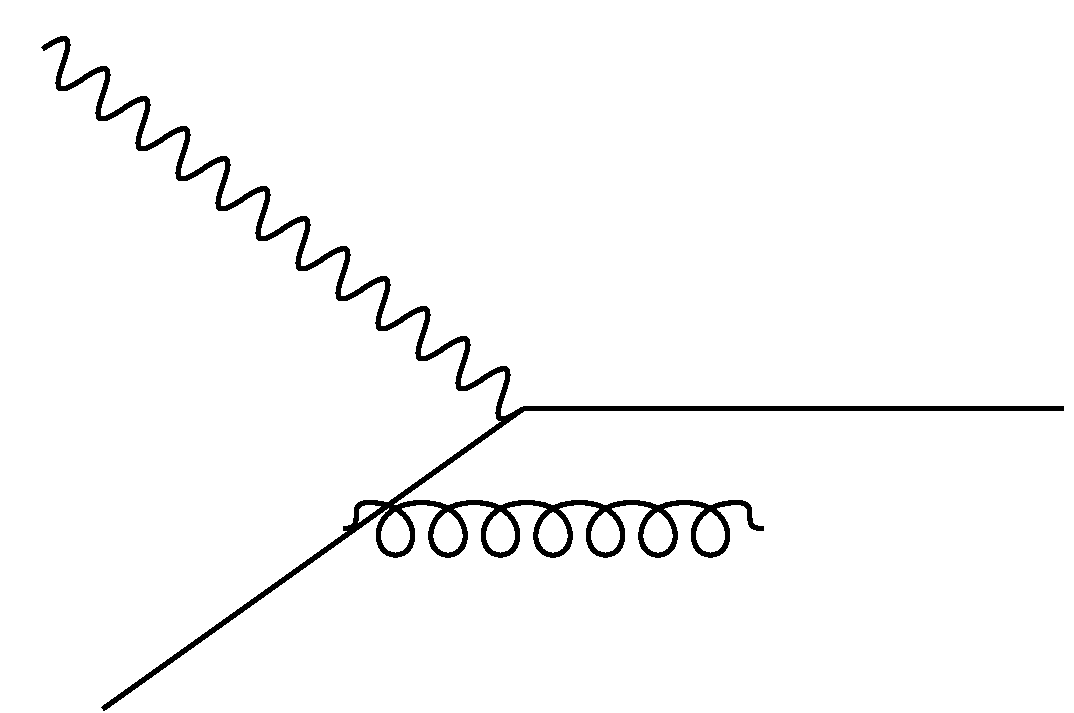
\includegraphics[scale=0.2]{real_initial_DIS.pdf}
    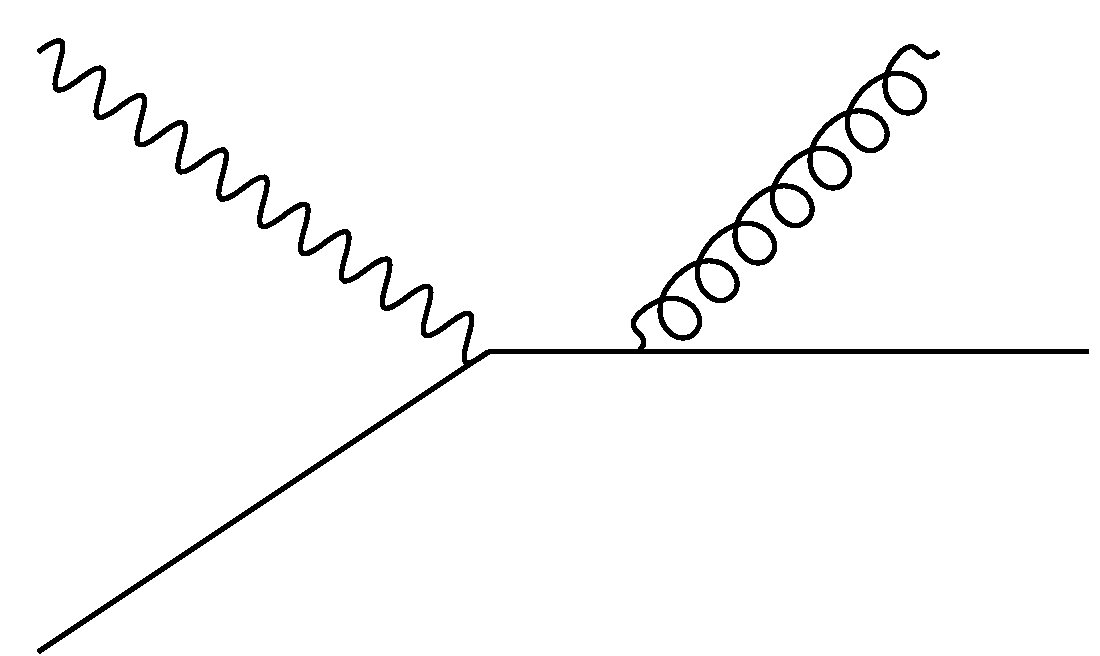
\includegraphics[scale=0.2]{real_final_DIS.pdf}
    \caption{Real NLO QCD corrections.}
    \label{fig:NLO_QCD_DIS}
\end{figure}

%
Working in a light-cone gauge, such logarithmic divergence can be traced back to the square of the amplitude associated
to a gluon emission from the initial state quark.
It can be shown, that denoting as $k_{\perp}$ the longitudinal momentum of the emitted gluon,
we end up with a contribution of the form
\begin{align}
    \label{eq:collinear_div}
    \hat{F}_{q\, \gamma \rightarrow q\,g}\left(x,Q^2\right) =
    \int^{\,Q^2}\frac{dk_{\perp}^2}{k_{\perp}^2}\, \alpha_s\, P\left(x\right) + ...\,,
    %\sim \alpha_s\left(Q^2\right)\,\log\frac{Q^2}{Q_0^2}\,,
\end{align}
where the ellipses stand for finite regular terms.
It is clear from Eq.~\ref{eq:collinear_div} that such term diverges in the region of small-$k_{\perp}$.
In order to regularize such pole we can introduce the infrared cutoff $Q_0^2$, getting the logarithmic 
contribution observed in Eq.~\ref{eq:1_loop_dis}.
Similarly, when considering multiple gluons emissions from initial state particles, terms of the kind 
$\left(\alpha_s\left(Q^2\right)\,\log\frac{Q^2}{Q_0^2}\right)^n$ show up.
Since all these terms are of order 1, if we accounted for only some of them we would spoil perturbation theory.
In order to get a proper perturbative expansion such terms have to be resummed at all orders.
Such resummation is achieved through factorization of collinear singularities into the parton model PDFs,
as described in the next section.

\subsection{Factorization of collinear singularities}
The singularities described in the previous sections arises from the kinematic region where $k_{\perp}\rightarrow 0$,
namely when a gluon is emitted parallel to an initial state quark. For this reason they are often called collinear
singularities.
To understand how to deal with such terms, one needs to realize that the limit of small$-k_{\perp}$
corresponds to the long-range (low energy) regime of the strong interaction and therefore cannot be treated
within perturbation theory.
We can then consider the parton distributions introduced through the parton model as bare, unmeasurable
quantities, and use them to reabsorb the collinear singularities. In this way, all the dependence on
low energy phenomena can be factorized in the parton distribution functions, leaving the hard
cross sections free from collinear singularities.

%
Starting from the logarithmic divergent contribution appearing in Eq.~\eqref{eq:1_loop_dis}, we can introduce an
additional unphysical scale $\mu_F$ and write
$\log\frac{Q^2}{Q_0^2} = \log\frac{Q^2}{\mu_F^2} + \log\frac{\mu_F^2}{Q_0^2} $.
Looking back at Eq.~\eqref{eq:strcuture_function},
the infrared divergent partonic structure function can then be written as
\begin{align}
  \label{eq::IRsubtraction}
  \hat{F}\left(\xi,Q\right) = 
  \int_{\xi}^1 \frac{d\eta}{\eta} \,\Gamma\left(\frac{\xi}{\eta},\mu_F\right)
  \hat{F}_{\text{reg}}\left(\eta,\frac{Q}{\mu_F}\right) ,
\end{align}
with
\begin{align}
    &\Gamma\left(y,\mu_F\right) = \delta\left(1-y\right) 
    + \alpha_s\left[P\left(y\right)\log\frac{\mu_F^2}{Q_0^2} + \Gamma_{finite}\left(y\right)\right]\,, \\
    &\hat{F}_{\text{reg}}\left(\eta,\frac{Q}{\mu_F}\right) = \delta\left(1-\eta\right)  
    + \alpha_s
    \left[P\left(\eta\right)\log\frac{Q^2}{\mu_F^2}+ R\left(\eta\right) - \Gamma_{finite}\left(\eta\right) \right]\,.  
\end{align}
The new scale $\mu_F$ introduced above, often referred to as factorization scale, separates long and short distance 
contributions: everything which is below $\mu_F$ is considered to be in a non perturbative regime 
and it is factorized in the kernel $\Gamma$, which therefore contains the infrared poles.
The term $\Gamma_{finite}$ represents finite contributions that can be
kept into the subtraction kernel rather than in the hard structure function. Its specific choice is what defines
the renormalization scheme.  
Substituting Eq.~\eqref{eq::IRsubtraction} in Eq.~\eqref{eq:strcuture_function} it is easy to see that
we can write
\begin{align}
  F\left(x,Q\right) = \sum_a\int_x^1 \frac{d\eta}{\eta}\, 
  q_{a/H}\left(\eta,\mu_F\right)\hat{F}_{\text{reg}}\left(\frac{x}{\eta},\frac{Q}{\mu_F}\right),
\end{align}
where the renormalized quark PDFs $q_{a/H}$ is defined as
\begin{align}
    \label{eq:renormalized_pdf}
    q_{a/H}\left(x,\mu_F\right) = \int_x^1 \frac{d\eta}{\eta} \,
    q^{\bare}_{a/H}\left(\frac{x}{\eta}\right)\Gamma\left(\eta, \mu_F\right)\,.
\end{align}
Collinear poles are therefore factorized from the hard scattering structure function and reabsorbed into
the PDFs, following a procedure symilar to the one used for UV renormalization.
As a consequence PDFs acquire a non trivial dependence on an unphysical scale $\mu_F$,
which will be further described in in the next section.

%
To sum up, considering higher orders QCD corrections, the DIS structure functions can be written
as
\begin{align}
    \label{eq:dis_qcd}
    F\left(x,Q^2\right) = 
    \sum_a \int_x^1\frac{d\xi}{\xi}\,C_a\left(\frac{x}{\xi},\frac{Q^2}{\mu_F^2}, \alpha_s\right)q_{a/H}\left(\xi,\mu_F^2\right)
    +\mathcal{O}\left(\frac{\Lambda_{QCD}}{Q}\right)\,.
\end{align}
The coefficients functions $C_a$ appearing in Eq.~\eqref{eq:dis_qcd} correspond to the finite partonic structure 
functions $\hat{F}_{\text{reg}}$ after renormalization and subtraction of collinear singularities.
Their explicit expression will depend on the specific structure function under consideration
and on the choice for the renormalization and factorization schemes, defined when removing UV and collinear
singularities respectively. 
Once properly defined they can be computed order by order in perturbation theory as an expansion in the strong coupling
\begin{align}
    \label{eq:coeff_functions_expansion}
    C_a\left(x, \alpha_s\right) = C_a^{(0)}\left(x\right) + \alpha_s\, C_a^{(1)}\left(x\right) 
    + \alpha_s^2\, C_a^{(2)}\left(x\right) + ...\,,
\end{align}
where the first contribution (LO) recover the parton model predictions, the second one (NLO) corresponds to the QCD
corrections discussed above and the coming ones (N$^{\text{n}}$NLO) will refer to higher order corrections.
Differently from the initial formula of Eq.~\eqref{eq:strcuture_function}, which was written in analogy to
the parton model formulation, the parton distributions
have now acquired a scale dependence, which cancel against an analogue dependence in the coefficient functions,
leaving the physical structure function independent from any unphysical scales. Also, even if in our 
discussion we have only considered the quark channel, the sum over the flavour types $a$ now includes
also gluon initiated contributions, which formally start at NNLO.

%
So far we have discussed factorization for processes with only one hadron in the initial state, but
the same ideas and logic apply to inclusive enough high-energy hadron-hadron collisions
$$
H_1\left(p_1\right) + H_2\left(p_2\right) \rightarrow W\left(Q\right) + X\,,
$$
where $H_1$ and $H_2$ are the incoming hadrons, having momenta $p_1$ and $p_2$, $H$ represents
the particle produced in the hard scattering (Higgs or vector bosons, heavy quarks) and $W$
denotes any other particle appearing in the final state. In this case the factorization formula takes the form
\begin{align}
    \label{eq:hadron_hadron}
    \sigma&\left(p_1,p_2,Q\right) = \sum_{a,b}\int_{\tau}^1\, 
    dx_1 dx_2 \, \nonumber \\ 
    &q_{a/H_1}\left(x_1,\mu_F^2\right)q_{b/H_2}\left(x_2,\mu_F^2\right)
    \hat{\sigma}_{ab}\left(x_1p_1,x_2p_2,\frac{Q^2}{\mu_F^2},\alpha_s\right) 
    + \mathcal{O}\left(\frac{\Lambda_{QCD}}{Q}\right)\,,
\end{align}
where $\tau = \frac{Q^2}{s}$ and $s=\left(p_1+p_2\right)^2$.

%
The two factorized expressions given in Eqs.~\eqref{eq:dis_qcd},~\eqref{eq:hadron_hadron}
allow to connect cross sections for high-energy processes having hadrons in the initial states to hard scattering processes.
The former can be measured in collider experiments, while the latter 
can be computed in perturbation theory. The objects connecting perturbation theory with physical observables are
the Parton Distribution Functions.
The content of the factorization theorem is that all the dependence
on low mass phenomena is entirely contained in the PDFs. Therefore, since they describe the internal structure 
of a given kind of hadron and have been decoupled from the short-distance details of
the specific process we consider, they are nonpertubative and universal objects.
This means that the PDFs appearing in the case of DIS must be the same considered for 
any other high-energy collisions.

%%%%%%%%%%%%%%%%%%%%%%%%%%%%%%%%%%%%%%%%%%%%%%%%%%%%
\section{Parton Distribution Functions}
In the previous section we have introduced PDFs as some bare objects,
which are then used to reabsorb the infrared collinear poles coming from the fixed order computation of partonic
hard cross sections. Following this approach PDFs are introduced in the discussion through 
the parton model ideas, and defined as objects containing all the dependence 
of the physical observable on low energy physics. 
%
It is possible to give a rigorous operator definition of parton distributions,
which can be applied beyond perturbation theory and makes manifest the universal nature of PDFs.
The formalism and notations commonly used to describe PDFs in terms of QCD operators are usually quite different
from those introduced in the previous section, which are commonly adopted for phenomenological applications.
Since in this work we will present results for which both formalism are required,
in this section we briefly revise the formal definition of PDFs, addressing their UV renormalization
and renormalization group equation and making contact with the formalism and notations introduced in the previous section.

\subsection{PDFs operator definition}
Working in the Bjorken limit, it can be proved~\cite{Collins:1980ui,Collins:1981uw} that the bare unpolarized 
quark PDF appearing in Eq.~\eqref{eq:strcuture_function} is related to the light-cone Fourier transform 
of a bilocal operator, given by
\begin{align}
	\label{eq::barepdf}                                                  
	f_\mathrm{q}^\bare\lp x \rp = \int \frac{d\xi^-}{4\pi} e^{-ixP^+\xi^-} 
	\langle \text{P}|\bar{\psi}_\mathrm{q}^\bare\lp\xi^-\rp\gamma^+ \,   
	U\lp\xi^-,0\rp \psi_\mathrm{q}^\bare\lp 0\rp  |\text{P}\rangle\, ,   
\end{align}
where $|\text{P}\rangle$ denotes a hadronic state with momentum $P^\mu = \lp
P^0,0,0,P^z\rp$, $x$ belongs to the real interval $\left[-1,1\right]$ and $P^{\pm}=\frac {\lp P^0 \pm P^z \rp}{ \sqrt{2}}$ are
light-cone coordinates. 
The index $\mathrm{q}$ identifies the parton under
investigation. For instance, in a theory where we only consider the four
lightest quarks, we have $q=u,d,s,c$. The momentum carried by the parton is
$k^\mu = x P^\mu$, $\psi_\mathrm{q}^\bare$ is the bare quark field operator and the
Wilson line $U$ is given by 
\begin{align}
	\label{eq::wilsonline}                                                      U\lp\xi^-,0\rp = \text{P}\exp 
    \lp -ig\int_0^{\xi^-}d\eta^- A^{\bare\,+}\lp \eta^- \rp \rp\, .         
\end{align}
An analogous definition can be given for the gluon bare PDFs, denoted as
$f_g^\bare\lp x \rp$. The superscripts $\bare$ in the above expressions identify
bare fields: the matrix elements that enter in the definition of
$f_\mathrm{q}^\bare$ are ultraviolet divergent, and therefore need to be
renormalized.
Renormalized parton distributions are usually defined by minimal
subtraction, and the relation between the bare and the renormalized quantities
is given by
\begin{align}
	\label{eq:RenormPDF}                                   
	f_a^\bare\lp x \rp = \sum_{b}\int_x^1\frac{dy}{y}\,\text{Z}_{ab}\lp\frac{x}{y},\mu \rp f_b\lp y,\mu^2 \rp\, , 
\end{align}
where the indices $a$ and $b$ run over all the parton types (gluon and flavors
of quarks) and $\mu$ denotes the renormalization scale introduced by the minimal
subtraction scheme. 

Focusing on the quark PDFs for now, the renormalized distributions introduced
above have a compact support given by the interval $[-1,1]$. 
To recover the conventions of the previous sections, used for
phenomenological applications, it is customary to define the PDFs on the
interval $[0,1]$, and to introduce independent functions for the quarks and the
antiquarks, which we have previously denoted as $q(x,\mu^2)$ and $\bar{q}(x,\mu^2)$ respectively.
The relation between $f_q$, $q$ and $\bar{q}$ is 
\begin{equation}
    \label{eq:DefFQQbar}
    f_\mathrm{q}\lp x,\mu^2\rp = 
    \begin{cases}
        \phantom{-}q(x,\mu^2)\, , &\quad \mathrm{if}\ x>0\, , \\
        -\bar{q}(-x,\mu^2)\, , &\quad \mathrm{if}\ x<0 \, .
    \end{cases}
\end{equation}
It is useful to consider the symmetrised and antisymmetrised combinations of
$f_\mathrm{q}$ in the interval $x\in[0,1]$:
\begin{eqnarray}
	\label{eq:fsym}
	f^\mathrm{sym}_\mathrm{q}(x,\mu^2)  &= f_\mathrm{q}(x,\mu^2) + f_\mathrm{q}(-x,\mu^2) 
	\, , \\
	\label{eq:fasym}
	f^\mathrm{asy}_\mathrm{q}(x,\mu^2)  &= f_\mathrm{q}(x,\mu^2) - f_\mathrm{q}(-x,\mu^2) \, .
\end{eqnarray}
It can be readily shown that
\begin{align}
    f^\sym_\mathrm{q}(x,\mu^2) &= 
    q(x,\mu^2) - \bar{q}(x,\mu^2) = q^-(x,\mu^2) \, , \\
    f^\asy_\mathrm{q}(x,\mu^2) &= 
    q(x,\mu^2) + \bar{q}(x,\mu^2) = q^+(x,\mu^2) \, .
\end{align}
where $q^+$ and $q^-$ are defined by the equations above. The flavor
decomposition can be rewritten by collecting the quark fields in a vector, \eg\
$\psi = \lp \psi_u,\psi_d,\psi_s,\psi_c\rp$, and defining the following nonsinglet bare
PDFs:
% \begin{eqnarray}
%     \label{eq:f3Def}
%     f_3^\bare(x) &= \int \frac{d\xi^-}{4\pi} e^{-ixP^+\xi^-} 
% 	\langle \text{P}|\bar{\psi}^\bare\lp\xi^-\rp \lambda_3 \gamma^+ \,   
% 	U\lp\xi^-,0\rp \psi^\bare\lp 0\rp  |\text{P}\rangle\, ,  \\
%     \label{eq:f8Def}
%     f_8^\bare(x) &= \int \frac{d\xi^-}{4\pi} e^{-ixP^+\xi^-} 
% 	\langle \text{P}|\bar{\psi}^\bare\lp\xi^-\rp \lambda_8 \gamma^+ \,   
% 	U\lp\xi^-,0\rp \psi^\bare\lp 0\rp  |\text{P}\rangle\, ,  \\
%     \label{eq:f15Def}
%     f_{15}^\bare(x) &= \int \frac{d\xi^-}{4\pi} e^{-ixP^+\xi^-} 
% 	\langle \text{P}|\bar{\psi}^\bare\lp\xi^-\rp \lambda_{15} \gamma^+ \,   
% 	U\lp\xi^-,0\rp \psi^\bare\lp 0\rp  |\text{P}\rangle\, ,  
% \end{eqnarray}
\begin{eqnarray}
    \label{eq:fADef}
    f_A^\bare(x) &= \int \frac{d\xi^-}{4\pi} e^{-ixP^+\xi^-} 
	\langle \text{P}|\bar{\psi}^\bare\lp\xi^-\rp \lambda_A \gamma^+ \,   
	U\lp\xi^-,0\rp \psi^\bare\lp 0\rp  |\text{P}\rangle\, , 
\end{eqnarray}
where $A=3,8,15$, and we have used the Gell-Mann matrices
\begin{eqnarray}
    \lambda_3=
    \begin{pmatrix}
        1 & 0 & 0 & 0\\
        0 & -1& 0 & 0\\
        0 & 0 & 0 & 0\\
        0 & 0 & 0 & 0
    \end{pmatrix}\, , \quad
    \lambda_8=
    \begin{pmatrix}
        1 & 0 & 0 & 0\\
        0 & 1& 0 & 0\\
        0 & 0 & -2 & 0\\
        0 & 0 & 0 & 0
    \end{pmatrix}\, , \quad
    \lambda_{15}=
    \begin{pmatrix}
        1 & 0 & 0 & 0\\
        0 & 1& 0 & 0\\
        0 & 0 & 1 & 0\\
        0 & 0 & 0 & -3
    \end{pmatrix}\, . 
\end{eqnarray}
In this notation $f_3$ corresponds to $f^{u-d}=f_u-f_d$, $f_8=f^{u+d-2s}$, and
so on. The symmetrised and antisymmetrised combinations map directly into the
so-called {\em evolution basis} for the PDFs that is normally used in
phenomenological studies, see \eg\ Ref.~\cite{Vogt:2004ns} for a detailed
definition of the flavor decomposition. More specifically, we have:
\begin{align}
    f^\asy_{3}  &= u^+ - d^+ = T_3 \, , \\
    f^\sym_{3}  &= u^- - d^- = V_3 \, , \\
    f^\asy_{8}  &= u^+ + d^+ - 2 s^+ = T_8 \, , \\
    f^\sym_{8}  &= u^- + d^- - 2 s^- = V_8 \, , \\
    f^\asy_{15} &= u^+ + d^+ + s^+ - 3 c^+ = T_{15} \, , \\
    f^\sym_{15} &= u^- + d^- + s^- - 3 c^- = V_{15} \, .
\end{align}

%
As mentioned above the bilocal operator products of Eq.~\ref{eq::barepdf} requires renormalization.
The corresponding renormalization group equations are the Altarelli-Parisi equations fo PDFs.
Considering on-shell incoming partons, a straightforward 1-loop computation gives
\begin{align}
    \label{eq:1-loop_bare_partonic_pdf}
    f^{\bare}_{a/b}\left(x,\epsilon\right) = \delta_{ab}\,\delta\left(1-x\right)
    + \alpha_s\left[\frac{1}{\epsilon_{UV}}-\frac{1}{\epsilon_{IR}}\right] P_{a/b}^{(1)}\left(x\right)
    + \mathcal{O}\left(\alpha_s^2\right)\,.
\end{align}
To obtain such result, one has to work in dimensional regularization to regularize both UV and infrared
divergences. 
Working in $\overline{MS}$ the UV pole $1/\epsilon_{UV}$ is removed through renormalization,
and we are left with the renormalized partonic PDFs
\begin{align}
    \label{eq:1-loop_renormalized_partonic_pdf}
    f_{a/b}\left(x,\epsilon\right) = \delta_{ab}\,\delta\left(1-x\right)
    + \alpha_s\left(-\frac{1}{\epsilon}\right) P_{a/b}^{(1)}\left(x\right)
    + \mathcal{O}\left(\alpha_s^2\right)\,.
\end{align}
Such object, despite being UV finite, does contain 
infrared poles.

%
We can now see how the formal approach followed here recovers the picture given in the previous section.
Taking as example the case of DIS structure function, we can apply Eq.~\ref{eq:dis_qcd} to the case of an 
incoming parton $b$\footnote{An important property of the hard coefficient functions is that they 
depend only on the parton type $a$ and not on the specific hadron $H$, 
so that they can be computed with the simplest choice of external parton.}
\begin{align}
    \label{eq:partonic_structure_function}
    \hat{F}_{b}\left(x,\epsilon\right) = 
    \sum_a \int_x^1\frac{d\xi}{\xi}\,C_a\left(\frac{x}{\xi}, \alpha_s\right)f_{a/b}\left(\xi,\epsilon\right)
    +\mathcal{O}\left(\frac{\Lambda_{QCD}}{Q}\right)\,.
\end{align}
Considering the coefficient functions power expansions given in Eq.~\eqref{eq:coeff_functions_expansion}
and an analogue expansion for $\hat{F}_{a}$, using the 1-loop expression for the
renormalized partonic PDF of Eq.~\eqref{eq:1-loop_renormalized_partonic_pdf} we get
\begin{align}
    \label{eq:IR_subtraction_from_formal_definition}
    &C^{(0)}_b\left(x\right) = \hat{F}_b^{(0)}\left(x\right)\,,\\
    &C^{(1)}_b\left(x\right) = \hat{F}_b^{(1)}\left(x,\epsilon\right) + \frac{1}{\epsilon}\sum_a\int_x^1 \frac{d\xi}{\xi}P_{a/b}^{(1)}\left(\xi\right)
    \hat{F}_a^{(0)}\left(\frac{x}{\xi}\right)\,,
\end{align}
which recovers the prescription introduced in the previous section: in order to compute
the hard scattering cross sections, one should calculate the structure function at the parton level and subtract
from it certain infrared divergent terms proportional to the splitting kernel and the Born cross section.
Such terms, identified as collinear emissions in the previous sections, here are computed in a process independent
way starting directly from the formal definition of PDFs.
Another way of stating this, is that the infrared subtraction kernel $\Gamma$ introduced in Eq.~\eqref{eq::IRsubtraction}
corresponds to the parton level renormalized PDF of Eq.~\eqref{eq:1-loop_renormalized_partonic_pdf}. For a proof
of this at every order in perturbation theory see for example \cite{Collins:1980ui}.


\subsection{DGLAP evolution equations}
\label{sec:DGLAP}
As stated in Eq.~\ref{eq:RenormPDF} the operator defining parton distribution functions requires
renormalization. As a consequence renormalized PDFs acquire a scale dependence.
Including in the discussion also the gluon PDF, the corresponding renormalization group equations read
\begin{align}
    \mu^2\frac{\partial}{\partial\mu^2}
    \begin{pmatrix}
        q_i\left(x,\mu^2\right) \\  
        g\left(x,\mu^2\right)
    \end{pmatrix}
    =
    \alpha_s\sum_{q_i,\bar{q}_i}\int_x^1 \frac{d\xi}{\xi} 
    \begin{pmatrix}
        P_{q_i q_j}\left(\frac{x}{\xi},\alpha_s\right) & P_{q_i g}\left(\frac{x}{\xi},\alpha_s\right) \\
        P_{g q_j}\left(\frac{x}{\xi},\alpha_s\right)   & P_{g g}\left(\frac{x}{\xi},\alpha_s\right) 
    \end{pmatrix}
    \begin{pmatrix}
        q_j\left(x,\mu^2\right) \\  
        g\left(x,\mu^2\right)
    \end{pmatrix}
\end{align}
with each splitting function computable in perturbation theory
\begin{equation}
    \begin{split}
    &P_{q_i q_j}\left(x,\alpha_s\right) = \delta_{ij}P^{(0)}_{qq}\left(x\right) 
    + \alpha_s P^{(1)}_{q_i q_j}\left(x\right) + ... \\
    &P_{q g}\left(x,\alpha_s\right) = P^{(0)}_{qg}\left(x\right) 
    + \alpha_s P^{(1)}_{q g}\left(x\right) + ... \\
    &P_{g q}\left(x,\alpha_s\right) = P^{(0)}_{gq}\left(x\right) 
    + \alpha_s P^{(1)}_{gq}\left(x\right) + ... \\
    &P_{g g}\left(x,\alpha_s\right) = P^{(0)}_{gg}\left(x\right) 
    + \alpha_s P^{(1)}_{gg}\left(x\right) + ... 
    \end{split}
\end{equation}
It is convenient to re-express the DGLAP equations choosing a PDFs basis which maximally diagonalize them. 
In order to do this the aforementioned evolution basis is particularly useful.
Denoting 
\begin{align}
    q^{\pm}_i = q_i \pm \bar{q}_i\,,
\end{align}
and considering the flavours $u, d, s, c, b, t$ the non-singlet sector is defined by the valence distributions
\begin{align}
    V_i = q_i^-
\end{align} 
and the $T_i$ combinations, defined as
\begin{align}
    T_3 = u^+ - d^+\,,\,\,\,\,\,\,T_8 = u^+ + d^+ -2s^+\,,\,\,\,\,\,\,T_{15} = u^+ + d^+ + s^+ -3c^+\,,\,\,\,\,\,\, \\
    T_{24} = u^+ + d^+ + s^+ + c^+ -4b^+\,,\,\,\,\,\,\, T_{35} = u^+ + d^+ + s^+ + c^+ + b^+ - 5 t^+\,. 
\end{align}
Each non-singlet distribution will then satisfy an independent evolution equation, given by 
\begin{align}
    \label{eq:DGLAP_NS}
    \mu^2\frac{d}{d\mu^2}q^{NS}\left(x,\mu^2\right) 
    = \int_{\xi}^1\frac{d\xi}{\xi}P\left(\xi,\alpha_s\right)
    q^{NS}\left(\frac{x}{\xi},\mu^2\right)\,.
\end{align}
The spitting function $P$ for $V_i$ and $T_i$ distributions is given by $P^-$ and $P^+$ respectively,
which at leading order are
\begin{align}
    P^{-(0)}\left(x\right) = P^{+(0)}\left(x\right) = \frac{C_F}{2\pi}\left(\frac{1+z^2}{1-z}\right)_+ \,.
\end{align}
Working in the evolution basis, the only distribution which couples to the gluon is the so called
singlet combination, defined as
\begin{align}
    \Sigma\left(x,\mu^2\right) = \sum_i \left(q_i\left(x,\mu^2\right)+\bar{q}_i\left(x,\mu^2\right)\right)
\end{align}
\begin{align}
    \mu^2\frac{\partial}{\partial\mu^2}
    \begin{pmatrix}
        \Sigma\left(x,\mu^2\right) \\  
        g\left(x,\mu^2\right)
    \end{pmatrix}
    =
    \alpha_s\int_x^1 \frac{d\xi}{\xi} 
    \begin{pmatrix}
        P_{q q}\left(\frac{x}{\xi},\alpha_s\right) & P_{q g}\left(\frac{x}{\xi},\alpha_s\right) \\
        P_{g q}\left(\frac{x}{\xi},\alpha_s\right)   & P_{g g}\left(\frac{x}{\xi},\alpha_s\right) 
    \end{pmatrix}
    \begin{pmatrix}
        \Sigma\left(x,\mu^2\right) \\  
        g\left(x,\mu^2\right)
    \end{pmatrix}
\end{align}
with the leading order splitting function given by
\begin{align}
    &P_{qq}^{(0)}\left(x\right) = \frac{C_F}{2\pi}\left[\frac{1+x^2}{\left(1-x\right)_+} 
    + \frac{3}{2}\delta\left(1-x\right)\right]\,,\nonumber \\
    &P_{gg}^{(0)}\left(x\right) = \frac{C_A}{\pi}\left[\frac{x}{\left(1-x\right)_+}
    + \frac{1-x}{x} + x\left(1-x\right)\right] 
    +\delta\left(1-x\right)\frac{\left(11C_A - 2n_f T_R\right)}{12\pi}\,, \nonumber \\
    &P_{gq}^{(0)}\left(x\right) = \frac{C_F}{2\pi}\left[\frac{1+\left(1-x\right)^2}{x}\right]\,, \nonumber \\
    &P_{qg}^{(0)}\left(x\right) = \frac{n_f}{2\pi}\left[x^2+\left(1-x\right)^2\right]\,.
\end{align}
Because of charge conjugation invariance and $SU(n_f)$ flavour symmetry splitting functions are independent on the quark
flavour and are the same for quarks and antiquarks. 
Also, leading order splitting function have a nice physical interpretation as probability distributions.
Following Ref.~\cite{ALTARELLI1977298}, Eq.~\ref{eq:DGLAP_NS} can be written as
\begin{align}
    q^{NS}&\left(x,\mu^2\right) + dq^{NS}\left(x,\mu^2\right) = \nonumber\\
    &\int_0^1 dy\int_0^1 dz\,\delta\left(zy-x\right) q^{NS}\left(y,\mu^2\right) 
    \left[\delta\left(z-1\right) + \alpha_s\, P\left(z\right) d \log\frac{\mu^2}{\mu_0^2}\right]\,.
\end{align}
The quantity in square brackets can then be interpreted as the probability density of finding a quark
inside another quark, with a fraction $z$ of the parent momentum. The quantity $\alpha_s P\left(z\right)$
is then the variation of such probability density per logarithmic unit of the energy. The interpretation
of splitting function as probability densities implies that they are positivite for $x<1$ and allows to compute
them starting from the QCD vertices for $q\rightarrow q\,g$, $g\rightarrow q\bar{q}$ and $g\rightarrow gg$.  

%
The QCD evolution equations can be solved computing an evolution kernel, which can be subsequently applied
to PDFs at a given scale $Q_0$ to evolve them up to the final scale $Q$.
In the following we briefly summarise how the QCD evolution equation can be solved for the
nonsinglet sector, yielding such evolution kernel.

Denoting the nonsiglet distributions $V_i$ and $T_i$ with $q^{(-)}$ and
$q^{(+)} $ respectively, the QCD evolution equations can be written as
\begin{align}
    \mu^2\frac{\partial }{\partial \mu^2} q^{(\pm)}\left(x,\mu^2\right) = 
    \frac{\alpha_s(\mu^2)}{2\pi}
    \int_{x}^{1}\frac{d\xi}{\xi}\, 
    P_{qq}^{(\pm)}\left(\frac{x}{\xi},\alpha_s(Q^2)\right)
    q^{(\pm)}\left(\xi,\mu^2\right),
\end{align}
which in Mellin space becomes
\begin{align}
\label{eq::dglapmellin}
    \mu^2\frac{\partial }{\partial \mu^2} q^{(\pm)}\left(N,\mu^2\right) = 
    \gamma^{(\pm)}\left(N, \alpha_s\right) q^{(\pm)}\left(N,\mu^2\right)\, .
\end{align}
The distribution at the scale $\mu^2$ is obtained from the distribution at the
scale $\mu_0^2$ by introducing the evolution operator $\Gamma$
\begin{align}
\label{eq::evolutionoperator}
    q^{(\pm)}\left(N,\mu^2\right) = 
    \Gamma^{(\pm)}\left(N,\alpha_s,\alpha_s^0\right)
    q^{(\pm)}\left(N,\mu_0^2\right)\, ,
\end{align}
where $\alpha_s \equiv \alpha_s\left(\mu^2\right)$ and $\alpha_s^0 \equiv
\alpha_s\left(\mu_0^2\right)$. Substituting Eq.~\eqref{eq::evolutionoperator} in
Eq.~\eqref{eq::dglapmellin} and remembering that the dependence of $\Gamma$ on
the scale $\mu$ is only through the coupling, we have
\begin{align}
\label{eq::Mdglap}
    \beta\left(\alpha_s\right) \frac{\partial}{\partial\alpha_s}
    \Gamma^{(\pm)}\left(N,\alpha_s,\alpha_s^0\right) = 
    \gamma^{(\pm)}\left(N, \alpha_s\right)
    \Gamma^{(\pm)}\left(N,\alpha_s,\alpha_s^0\right)\, .
\end{align}
%
Considering for example {\tt NLO} evolution equations using 
\begin{align}
    & \beta\left(\alpha_s\right) = \frac{d\alpha_s}{d\log \mu^2} = 
    -\alpha_s^2 \beta_0 -\alpha_s^3 \beta_1 + \mathcal{O}\lp \alpha_s^4 \rp  \\
    & \gamma^{(\pm)}\left(N, \alpha_s\right) = 
    \frac{\alpha_s}{4\pi} \gamma^{(\pm)}_0\left(N\right) + 
    \left(\frac{\alpha_s}{4\pi}\right)^2 \gamma^{(\pm)}_1\left(N\right) + \mathcal{O}\lp \alpha_s^3 \rp\, ,
\end{align}
we can solve Eq.~\eqref{eq::Mdglap}; the Mellin space expression for the evolution
kernel at {\tt NLO} is
\begin{align}
    \Gamma^{(\pm)}\left(N,\alpha_s,\alpha_s^0\right) = 
    1 + \frac{\alpha_s -\alpha_s^0}{4\pi}
    \left(\frac{\gamma^{(\pm)}_1 \left(N\right)}{2\beta_0} - 
    \frac{\beta_1 \gamma^{(\pm)}_0\left(N\right)}{2\beta_0^2}\right)
    \,.
\end{align}
%
The solution in the $x$-space is obtained by computing the inverse Mellin
transform of $\Gamma^{(\pm)}\left(N,\alpha_s,\alpha_s^0\right)$. Having
analytically continued the function $\Gamma\left(N\right)$ to the complex plane,
the inverse Mellin transform is obtained by computing the contour integral
\begin{align}
    \Gamma^{(\pm)}\left(x,\alpha_s,\alpha_s^0\right) = 
    \int_C \frac{dN}{2\pi i}x^{-N}\, 
    \Gamma^{(\pm)}\left(N,\alpha_s,\alpha_s^0\right)\, .
\end{align}

% \comment{TG: this part can probably be removed, giving just the reference to the old nnpdf publication..?}
% We follow the approach implemented and validated in Ref.\cite{DelDebbio:2007ee}, reported here for completeness.
% The contour integral is computed choosing the Talbot path
% \begin{align}
% N\left(\theta_k\right)= r\theta/\left(1/\tan\theta + i\right),\,\,\,\,\,\,\,\,-\pi < \theta <\pi,
% \end{align}
% and using the Fixed Talbot algorithm, getting the expression
% \begin{align}
% \Gamma\left(x\right)= \frac{r}{M}\left[\frac{1}{2}\Gamma\left(N=r\right)x^{-r}+\sum_{k=1}^{M-1}\text{Re}\left[x^{-N\left(\theta_k\right)}\Gamma\left(N\left(\theta_k\right)\right)\left(1+i\sigma\left(\theta_k\right)\right)\right],\right]
% \end{align}
% with
% \begin{align}
% &\sigma\left(\theta\right) = \theta + \left(\theta/\tan\theta-1\right)/\tan\theta \\
% &\theta_k = \frac{k\pi}{M} \\
% &r = 2M/(5 \log\frac{1}{x})
% \end{align}
% where M is taken equal to 16.


\section{Heavy quarks}
\label{sec:fonll}
Considering a process in perturbative QCD involving heavy quarks\footnote{considering a process 
characterized by an hard scale $Q^2$,
we define a quark to be heavy if $m_h^2\gg Q^2$, with $m_h$ the quark mass. 
This definition is usually applied to the charm, bottom and top quarks.}, the corresponding cross-section
can be computed  in different renormalization schemes. In a standard minimal subtraction scheme, like $\overline{MS}$,
heavy quarks are treated on the same footing
as light flavours. 
In practise this means two things: first, they are endowed with a PDF and second 
the $\beta$ function depends on the total number $n_f$ of both light and heavy flavours. 
Alternatively, in a decoupling scheme heavy quarks are treated as massive particles 
which fully decouple from QCD evolution equations, 
so that only the $n_l$ light quarks contribute to the DGLAP and running of $\alpha_s$.
In the first case, often denoted as massless scheme, collinear logarithms of $Q^2/m_h^2$
are resummed through DGLAP equations and reabsorbed in the corresponding PDF, but corrections
suppressed by powers of $m_h^2/Q^2$ are neglected.
In the second option, denoted as massive scheme, collinear logarithms are only included to fix order, but the 
full mass dependence is retained.
While a minimal subtraction scheme is more precise at high scales $Q^2 \gg m_h^2$, where unresummed collinear logarithms
would spoil perturbation theory, a decoupling scheme is more accurate close to the threshold, where mass
corrections might be non negligible.
Heavy quarks schemes are all based on the idea of combining these two computations, each of which is more accurate 
in a certain kinematic region, in order to get a single result which is accurate at all scales.
Some of the possible options available from the literature are 
the ACOT \cite{Aivazis:1993pi, Aivazis:1993kh, Tung:2001mv}, S-ACOT \cite{Kramer:2000hn}, TR \cite{Thorne:1997ga}
and FONLL schemes.
The latter was initially introduce in Ref.~\cite{Cacciari:1998it} in the context of hadroproduction of heavy quarks, and subsequently 
extended to DIS structure functions in Refs.~\cite{Forte:2010ta} and to hadronic processes in Ref.~\cite{Forte:2015hba}.

%
In the following, using the notations of Refs.~\cite{Forte:2010ta,Forte:2015hba} we will briefly recall 
the main features of the FONLL scheme, which will be used in
Chapter~\ref{ch:bottom} to construct a new method to deal with initial state heavy quarks in an hadronic process.
Assuming an hadronic process involving $n_l$ light quarks $q$  and only one massive quark $h$ of mass $m_h$,
the corresponding cross section in the massless $(n_l+1)$-flavours scheme is given by
\begin{align}
    \label{eq:massless}
    \sigma^{(n_l+1)} = \int \int dx_1 dx_2\, \sum_{ij=g,q,\bar{q},h,\bar{h}}&\, 
    f_i^{(n_l+1)}\left(x_1,\mu^2\right)f_j^{(n_l+1)}\left(x_2,\mu^2\right) \nonumber \\
    &\times\hat{\sigma}^{(n_l+1)}_{ij}\left(x_1,x_2,\alpha_s^{(n_l+1)}\right)\,.
\end{align}
The sum in Eq.~\ref{eq:massless} runs on both light and heavy flavours, which are all treated in the
$\overline{MS}$ scheme. The heavy quark has an associated PDF and contributes to both the
DGLAP evolution equation and to the running of $\alpha_s$, which is therefore denoted as $\alpha_s^{(n_l+1)}$. 
For simplicity we have omitted the
dependence on the factorization and renormalization scales in the hard cross section.
The same process can be computed in the massive $(n_l)$-flavours scheme as
\begin{align}
    \label{eq:massive}
    \sigma^{(n_l)} = \int \int dx_1 dx_2\, \sum_{ij=g,q,\bar{q}}&\, 
    f_i^{(n_l)}\left(x_1,\mu^2\right)f_j^{(n_l)}\left(x_2,\mu^2\right) \nonumber \\
    &\times\hat{\sigma}^{(n_l)}_{ij}\left(x_1,x_2,\frac{\mu^2}{m_h^2},\alpha_s^{(n_l)}\right)\,.
\end{align}
Unlike the case of the massless computation, here the sum is on light flavours only, there is no PDF corresponding
to the heavy quark and the hard cross-section retains the explicit dependence on the heavy quark mass $m_h$.
In order to match the two computations, we express Eqs.~\ref{eq:massless}, \ref{eq:massive} in terms of 
the massless schemes coupling $\alpha_s^{(n_l+1)}$ and light quarks PDFs $f^{(n_l+1)}_i$,
$i = g,q,\bar{q}$ using relations of the form
\begin{align}
    \label{eq:matching_alpha}
    &\alpha_s^{(n_l+1)}\left(\mu^2\right) = 
    \alpha_s^{(n_l)}\left(\mu^2\right) 
    + \sum_{k=2}^{\infty} c_k\left(L\right) \left(\alpha_s^{(n_l)}\left(m_h^2\right)\right)^k\,, \\
    \label{eq:matching_PDFs}
    &f_i^{(n_l+1)}\left(x_1,\mu^2\right) = \int_x^1 \frac{dy}{y} 
    \sum_{j=g,q,\bar{q}} K_{ij}\left(\frac{x}{y}, L, \alpha_s^{(n_l)}\left(\mu^2\right)\right) f_j^{(n_l)}\left(y,\mu^2\right)\,,
\end{align}
where $i = g, q, \bar{q}, h, \bar{h}$ and $L = \log \mu^2/m_h^2$. The coefficients $c_k\left(L\right)$ are polynomial in $L$,
and the functions $K_{ij}$ can be expressed as a power expansion in $\alpha_s$ with coefficients
that are polynomial in $L$. The sum over $j$ in Eqs.~\ref{eq:matching_PDFs}
runs over the $n_l$ light flavours and anti-flavour plus the gluon, therefore the first $2n_l+1$
of these equations relate the light quarks and gluon PDFs in the two schemes and can be inverted in
order to express the massive scheme PDFs in terms of the massless scheme ones. The last two equations
allow to express the heavy quark PDF in the massless schemes in terms of the gluon and light flavours PDFs of the massive one,
under the assumption that the heavy quark PDF is generated perturbatively.
%
Inverting Eq.~\ref{eq:matching_alpha},~\ref{eq:matching_PDFs} and substituting in Eq.~\ref{eq:massive},
one can obtain the expression of the massive scheme cross-section in terms of $\alpha_s^{(n_l+1)}$
and $f_i^{(n_l+1)}$, $i = g,q,\bar{q}$
\begin{align}
    \label{eq:massive_as_func_massless}
    \sigma^{(n_l)} = \int \int dx_1 dx_2\, \sum_{ij = g,q,\bar{q} }&\, 
    f_i^{(n_l+1)}\left(x_1,\mu^2\right)f_j^{(n_l+1)}\left(x_2,\mu^2\right) \nonumber \\
    &\times B_{ij}\left(x_1,x_2,\frac{\mu^2}{m_h^2},\alpha_s^{(n_l+1)}\right)\,.
\end{align}
From now on we can use Eq.~\ref{eq:massive_as_func_massless} to express the massive scheme results, avoiding
any further reference to $\alpha_s^{n_l}$ and $f_i^{(n_l)}$\footnote{Eqs.~\ref{eq:massive_as_func_massless}
differs from the original massive scheme expression Eq.~\ref{eq:massive} by subleading terms.}.
Using again Eqs.~\ref{eq:matching_PDFs} to express the massless scheme heavy quarks PDFs in terms of light-quark parton
distributions, the massless scheme results Eq.~\ref{eq:massless} can be written entirely in terms of 
light-quark PDFs
\begin{align}
    \label{eq:massless_1}
    \sigma^{(n_l+1)} = \int \int dx_1 dx_2\, \sum_{ij=g,q,\bar{q}}&\, 
    f_i^{(n_l+1)}\left(x_1,\mu^2\right)f_j^{(n_l+1)}\left(x_2,\mu^2\right) \nonumber \\
    &\times A_{ij}\left(x_1,x_2,L,\alpha_s^{(n_l+1)}\right)\,,
\end{align}
where the coefficients $A_{ij}$ are given by a perturbative expansion of the form
\begin{align}
    \label{eq:expansionA}
    A_{ij}\left(x_1,x_2,L,\alpha_s^{(n_l+1)}\left(\mu^2\right)\right)&
    = \sum_{p=0}^N \left(\alpha_s^{n_l+1}\left(\mu^2\right)\right)^p \nonumber\\
    &\times\sum_{k=0}^{\infty} A_{ij}^{(p),(k)}\left(x_1,x_2\right)\left(\alpha_s^{(n_l+1)}\left(\mu^2\right)L\right)^k\,,
\end{align}
where at leading order $N=0$, at N$^k$LO $N=k$.
On the other hand, also the coefficient functions $B_i$ admit a fixed order expansion in $\alpha_s^{(n_l+1)}$
\begin{align}
    \label{eq:massive_1}
    B_{ij}\left(x_1,x_2,\frac{\mu^2}{m_h^2},\alpha_s^{(n_l+1)}\left(\mu^2\right)\right)
    = \sum_{p=0}^P \left(\alpha_s^{(n_l+1)}\left(\mu^2\right)\right)^p B_{ij}^p\left(x_1,x_2,\frac{\mu^2}{m_h^2}\right)\,.
\end{align}
In order to match the two results given in Eqs.~\ref{eq:massless_1},~\ref{eq:massive_as_func_massless} 
one should notice that the contributions to the massive scheme expression of Eq.~\ref{eq:massive_1}
which do not vanish when $\mu^2 \gg m_h^2$, namely all the constant and logarithmic terms, 
must also be present in the massless scheme computation.
The $p$-th order contribution to the sum of these terms $B_i^{(0),\,p}$ can be defined as
\begin{align}
    \lim_{m_h\rightarrow 0}\left[B_{ij}^p\left(x_1,x_2,\frac{\mu^2}{m_h^2}\right)- 
    B_{ij}^{(0),\,p}\left(x_1,x_2,\frac{\mu^2}{m_h^2}\right)\right] = 0\,,
\end{align}
and since it has also to be present in the massless scheme computation it will admit an expansion of the form
\begin{align}
    \label{eq:expansionB0}
    B_{ij}^{(0),\,p}\left(x_1,x_2,,\frac{\mu^2}{m_h^2}\right) = \sum_{k=0}^p  A_{ij}^{(p-k),(k)}\left(x_1,x_2,\right)L^k\,.
\end{align}
The FONLL method can be expressed as follows: considering the massless scheme coefficients
at a given perturbative order $p$ $A^{(p),(k)}_{ij}$ 
appearing Eq.~\ref{eq:expansionA}, replace all the terms which are also present in the massless limit of the massive scheme
$B^{(0),p}_{ij}$ Eq.~\ref{eq:expansionB0} with their fully massive expression $B^{p}_{ij}$ appearing in Eq.~\ref{eq:massive_1}.
This can be done in a systematic way defining the massless limit of the massive computation as
\begin{align}
    \label{eq:massive_massless_limit}
    \sigma^{(n_l),(0)} = \int \int dx_1 dx_2\, \sum_{ij = g,q,\bar{q} }&\, 
    f_i^{(n_l+1)}\left(x_1,\mu^2\right)f_j^{(n_l+1)}\left(x_2,\mu^2\right) \nonumber \\
    &\times B^{(0)}_{ij}\left(x_1,x_2,\frac{\mu^2}{m_h^2},\alpha_s^{(n_l+1)}\right)\,,
\end{align}
with
\begin{align}
    B^{(0)}_{ij} = \sum_{p=0}^N \left(\alpha_s^{(n_l+1)}\right)^p  B_{ij}^{(0),\,p}\left(x_1,x_2,\frac{\mu^2}{m_h^2}\right)\,,
\end{align}
and computing 
\begin{align}
    \sigma^{FONLL} = \sigma^{(n_l+1)} + \sigma^{(n_l)} - \sigma^{(n_l),(0)}\,.
\end{align}
In this way the mass suppressed terms which are not included in a massless computation, but which
are known from the massive one, are included in the final results.
On the other hand the all order resummation of collinear logarithms $L$ achieved 
in a massless scheme through DGLAP equations, which would be lost in the massive scheme, is now taken into account.
\clearpage
\newpage
In the following I report a draft of the table of contents of my thesis.
For most of the sections I have already collected all the material I need, expect for some of the points of the third chapter,
which are still work in progress. However I have not started the proper writing of the thesis yet.

\begin{enumerate}
    \item Factorization theorems in QCD
    \begin{itemize}
        \item Basics of QCD: I will revise some basic notions of QCD, from the lagrangian to the running coupling.
        \item Factorization theorems in high-energy physics: I will revise and discuss the parton model and factorization theorems
        in high-energy physics, focusing on DIS and hadronic processes.
        \item Factorization for heavy quarks: I will discuss massive and massless schemes and the FONLL method in the computation of
        physical cross sections.
    \end{itemize}
    \item Towards NNPDF4.0
    \begin{itemize}
        \item Machine learning in physics: I will discuss applications of machine learning in physics,
        introducing a series of general concepts and techniques commonly used in AI literature.
        In order to do this I will present part of the work done in Ref.~\cite{Cossu:2018pxj}, where such
        tools have been applied to a statistical physics problem.
        I will then move to discuss how machine learning has been applied within the framework
        of high-energy physics, to determine PDFs within the NNPDF collaboration.
        \item N3fit development: I will present studies regarding the choice of basis and parameterization in a PDFs fit.
        I will also discuss the phenomenological impact of positivity and integrability constraints on PDFs.
        \item Theory uncertainty: I will discuss the treatment of theory uncertainty in a fit, with particular focus on the details 
        of its practical implementation. Based on \cite{AbdulKhalek:2019bux, AbdulKhalek:2019ihb}.
        \item New experimental data: I will present and discuss the impact of new experimental data within the standard NNPDF31 dataset,
        focusing on jets data. Based on \cite{AbdulKhalek:2020jut}.     
        \item A new treatment for the b-PDF: I will present an alternative treatment of the b-PDF, based on \cite{Forte:2019hjc}.
    \end{itemize}
    \item PDFs from lattice data
    \begin{itemize}
        \item Factorization for equal-time correlators: 
        I will discuss the basic theoretical ideas behind the extraction of PDFs from lattice QCD data, presenting
        the main points within the framework of a nongauge theory.
        A paper about this is in preparation.
        \item PDFs from q-PDFs data: I will discuss results regarding PDFs from quasi-PDFs lattice data. Based on \cite{Cichy2019}.
        \item PDFs from p-PDFs data: I will discuss results regarding PDFs from pseudo-PDFs lattice data. 
        A paper about this is in preparation.
        \item Towards a first global lattice QCD fit: I will discuss the possibility of performing a first global analysis 
        over lattice QCD data.
    \end{itemize}
\end{enumerate}
%\singlespace

%\phantomsection
%\addcontentsline{toc}{chapter}{\bibname}
% Choose a bibliography style to suit your taste here
% This one was downloaded from http://web.reed.edu/cis/help/latex/bibtexstyles.html (June 2012)
\bibliographystyle{UTPstyle}
\bibliography{main, chapter1/chapter1, chapter2/chapter2}

\end{document}
